\documentclass[smaller,table]{beamer} %use 'handout' option for handouts

\usetheme{clecturesty}

\subtitle{Lecture 1 of 5}

\begin{document}

{
\logo{\includegraphics[width=0.30\textwidth]{imperialblue}}
\begin{frame}
  \titlepage
\end{frame}
}

\section{Introduction}
\subsection{The Course}

\begin{frame}
\frametitle{Introduction to the Course}
This course has been adapted from its previous incarnation, run by Dr Steven Capper.
Originally the course was based on the C course run by Dan Moore. The original course material, which may be useful, can be found at
\url{http://www.ma.ic.ac.uk/~drmii}
\begin{block}<+->{Aims of the Course}
\begin{itemize}
\item To introduce C programming from scratch.
\item To provide insight into scientific computing.
\item To write fast, efficient, multi-threaded code!
\end{itemize}
\end{block}

\begin{block}<+->{Five afternoon lectures from 2:00-4:00}
\begin{itemize}
\item Each afternoon will consist of a $\approx 1$ hour lecture,
\item a 10 minute break,
\item an hour of practical work.
\end{itemize}
\end{block}
\end{frame}

\begin{frame}
\frametitle{Course Content}
\begin{block}<+->{What we'll cover}
\begin{itemize}
\begin{small}
\item Different number types in C (Integers and Floating Point).
\item Operators, operands and their precedence.
\item Conversions and casts.
\item Mathematical expressions.
\item Statements: choice, while, do-while, switch, for loops$\ldots$
\item Functions in C.
\item Pointers, arrays and matrices.
\item Characters, strings and interacting with the console.
\item Reading and writing files.
\item Scientific C-Libraries and their uses: NAG, GSL, etc.
\item C++ and other languages.
\item High Performance Computing.
\item An Introduction to Parallel Computing.
\end{small}
\end{itemize}
\end{block}
\end{frame}

\subsection{What is C}
\begin{frame}
\frametitle{A Rough History of C}
\begin{block}<+->{Invented $\approx{1970}$}
By Dennis Ritchie working in Bell Labs USA; to facilitate development of
a portable UNIX.
\end{block}
\begin{block}<+->{C has been standardised}
\begin{itemize}
\item 1989 ANSI standard ratified \emph{ANS X3.159-1989}.
\item 1990 ISO standard \emph{ISO/IEC 9899:1990}. Aka \emph{C90}.
\item 2000 ISO standard \emph{ISO/IEC 9899:1999}. Aka \emph{C99}.
\end{itemize}
\end{block}
\begin{block}<+->{C has evolved into C++}
Bjarne Stroustrup developed C++ (C with class). Unlike C, C++ is still under
very active development (TR1 being the most recent standard at the time of
writing).
\end{block}
\end{frame}

\begin{frame}
\frametitle{What are C and C++?}
\begin{itemize}
\item C is a cross-platform, compiled, general-purpose language.
\item C++ can loosely be thought of as C's object oriented big brother.
\end{itemize}
\begin{alertblock}<+->{}
The vast majority of the programs running on your computer (including the operating system kernel), are written in either C or C++.
\end{alertblock}
\end{frame}


\begin{frame}
\frametitle{Why Use C? (Over Maple, Matlab$\ldots$ Excel(?!)$\ldots$)}
\begin{block}<+->{Speed}
C programs are compiled to machine code, the resulting routines \emph{can} run several orders of magnitude quicker than their equivalents in interpreted environments.
\end{block}

\begin{block}<+->{Flexibility}
The C language is intrinsically low level, one can manipulate complex data structures with surprisingly little code.
\end{block}

\begin{block}<+->{Portability}
A well written C program can target many different environments (Windows PCs, Linux workstations, Apple Macs, DEC Alphas, Embedded devices, $\ldots$).
\end{block}
\end{frame}

\section{Getting Started}
\subsection{Software}
\begin{frame}
\frametitle{Getting Started}
You will need:
\begin{itemize}
\item A C compiler (many different ones to choose from, some are free).
\item Some documentation (such as the lecture notes/exercises from this course,
a good book, online guides).
\item Lots, and lots of time.
\end{itemize}
\end{frame}

\begin{frame}
\frametitle{C Compilers}
\begin{itemize}
\item {\tt Intel} - for Windows or Linux. Compiles highly optimised code for Intel (and AMD) processors. Free for personal use, academic/commercial licenses obtainable from:
\url{http://www.polyhedron.com}
\item{\tt Microsoft Visual Studio 2010 Professional} - Microsoft's flagship compiler. Ninety day free trial available at:
\url{http://www.microsoft.com/visualstudio/en-us/try}
\end{itemize}
\end{frame}

\begin{frame}
\frametitle{Free C Compilers}
\begin{block}<+->{Linux}
\begin{itemize}
\item {\tt gcc} - The GNU Compiler Collection, C compiler.
\url{http://gcc.gnu.org}.
\end{itemize}
\begin{block}<+->{Windows}
\begin{itemize}
\item {\tt Visual C++ 2010 Express} - Microsoft's free compiler,
\url{http://www.microsoft.com/express/vc/}
\item {\tt MinGW} - Minamilist GNU for Windows,
\url{http://www.mingw.org/}.
\end{itemize}
\end{block}
\end{block}
\end{frame}

\begin{frame}
\frametitle{Integrated Development Environments}
gcc (and MinGW) are command line driven compilers; an Integrated Development Environment (IDE) is a graphical application that provides tools to assist with editing, compiling and debugging of code. I'd recommend Visual Studio Professional as an IDE, this can be obtained through DreamSpark if you're eligible. For a non-windows or free alternative, I'd recommend:
\begin{block}{}
\begin{description}
\item[Windows] \texttt{Visual C++ 2010 Express}, the free Microsoft IDE. \url{http://www.microsoft.com/express/vc/}
\item[Linux/Mac/Windows (free)] \texttt{Code::Blocks}, a cross-platform, open source IDE. \url{http://www.codeblocks.org/}
\item [Macs] \texttt{Xcode Tools}, the development environment used by Apple. \url{http://developer.apple.com/technology}
\end{description}
\end{block}
\end{frame}

\subsection{Books}
\begin{frame}
\frametitle{Books for C}
\begin{block}<+->{Kernighan and Ritchie (K\&R2)}
\begin{columns}
\begin{column}{1.5cm}

\includegraphics[width=\textwidth]{kandr.png}
\end{column}
\begin{column}{8cm}
\emph{The C Programming Language}, {\emph Second Edition},
Prentice Hall. \textbf{The} C reference.
\end{column}
\end{columns}
\end{block}

\begin{block}<+->{\emph{Numerical Recipes in C}}
\begin{columns}
\begin{column}{1.5cm}
\includegraphics[width=\textwidth]<2>{nr.png}
\end{column}
\begin{column}{8cm}
By Press, Teukolsky, Vetterling \& Flannery, {\emph Second Edition}, CUP.
Full of high quality example scientific C code. A free online edition can be found at:
\url{http://www.nr.com}\\*There is also a C++ edition in paper or online format.
\end{column}
\end{columns}
\end{block}
\end{frame}

\subsection{Building a C Program}
\begin{frame}
\frametitle{Building a C Program}
\begin{itemize}
\item To \emph{build} an executable from source, we carry out the following
three steps:
\begin{columns}
\begin{column}{3.1cm}
\begin{block}<+->{Edit Source}
Use a text editor to create a {\tt .c} file.
\end{block}
\end{column}
\begin{column}{3.8cm}
\begin{block}<+->{Compile}
With a C compiler, this creates \emph{object file(s)}.
\end{block}
\end{column}
\end{columns}
\begin{columns}
\begin{column}{3.8cm}
\begin{block}<+->{Link}
Combine the object files together into an \emph{executable}.
\end{block}
\end{column}
\end{columns}
\vspace{0.2in}
\item<+-> These steps are can be automated by \emph{Integrated Development Environments}
(IDEs).
\end{itemize}
\end{frame}

\section{Writing C}
\subsection{Hello World}
\ifhandout
\begin{frame}[fragile]
\frametitle{The Traditional Way to Start}
\begin{semiverbatim}
\kr\kl\kw{#include} \kt{<stdio.h>}
\kl
\kl\kw{int} main(\kw{void})
\kl\{
\kl   printf(\kt{"Hello World!\\n"});
\kl   \kw{return} 0;
\kl\}
\end{semiverbatim}

\begin{block}{The ``Hello World'' Program}
A traditional first program started by Ritchie. This is one of the smallest possible C programs that demonstrates some functionality (printing to screen).
\end{block}

\begin{block}{Line 1}
A \emph{pre-processor directive} (it begins with a {\tt \#}) advertising extra routines to the compiler.
\end{block}
\end{frame}

\begin{frame}
\begin{block}{Line 2}
An empty line, or equivalently, a line consisting solely of \emph{whitespace}. This is ignored by the compiler but makes the source code more readable.\end{block}

\begin{block}{Line 3}
A \emph{function declaration}, defining our {\tt main} function. The
{\tt main} function is where our program starts and is known as an
\emph{entry point}. Our main function takes \emph{no parameters} (\kw{\tt void}) and \emph{returns} an integer (\kw{\tt int}).
\end{block}

\begin{block}{Line 4}
\emph{Opening brace}, all statements enclosed between the braces {\tt\{}, {\tt\}} belong to the {\tt main} function.
\end{block}

\end{frame}

\begin{frame}
\begin{block}{Line 5}
A \emph{statement}; the \kw{\tt printf} (print formatted) function is called with the argument \kt{\tt "Hello World!$\backslash$n"}. This prints:\\
{\tt Hello World!}\\
to \emph{standard output} (usually a text console).
\end{block}

\begin{block}{Line 6}
A \emph{return statement}, we exit {\tt main} with a return code of 0. The system interprets 0 as ``success''.
\end{block}


\begin{block}{Line 7}
A \emph{closing brace}, everything after this line does not belong to
{\tt main}.
\end{block}

\end{frame}

\else
\begin{frame}[fragile]
\frametitle{The Traditional Way to Start}
\begin{semiverbatim}
\alert<2>{\kr\kl\kw{#include} \kt{<stdio.h>}}
\alert<3>{\kl}
\alert<4>{\kl\kw{int} main(\kw{void})}
\alert<5>{\kl\{}
\alert<6>{\kl   printf(\kt{"Hello World!\\n"});}
\alert<7>{\kl   \kw{return} 0;}
\alert<8>{\kl\}}
\end{semiverbatim}

\only<1>{\begin{block}{The ``Hello World'' Program}
A traditional first program started by Ritchie. This is one of the smallest possible C programs that demonstrates some functionality (printing to screen).
\end{block}
}

\only<2>{\begin{block}{Line 1}
A \emph{pre-processor directive} (it begins with a {\tt \#}) advertising extra routines to the compiler.
\end{block}}

\only<3>{\begin{block}{Line 2}
An empty line, or equivalently, a line consisting solely of \emph{whitespace}. This is ignored by the compiler but makes the source code more readable.\end{block}
}

\only<4>{\begin{block}{Line 3}
A \emph{function declaration}, defining our {\tt main} function. The
{\tt main} function is where our program starts and is known as an
\emph{entry point}. Our main function takes \emph{no parameters} (\kw{\tt void}) and \emph{returns} an integer (\kw{\tt int}).
\end{block}
}

\only<5>{\begin{block}{Line 4}
\emph{Opening brace}, all statements enclosed between the braces {\tt\{}, {\tt\}} belong to the {\tt main} function.
\end{block}
}

\only<6>{\begin{block}{Line 5}
A \emph{statement}; the \kw{\tt printf} (print formatted) function is called with the argument \kt{\tt "Hello World!$\backslash$n"}. This prints:\\
{\tt Hello World!}\\
to \emph{standard output} (usually a text console).
\end{block}
}

\only<7>{\begin{block}{Line 6}
A \emph{return statement}, we exit {\tt main} with a return code of 0. The system interprets 0 as ``success''.
\end{block}
}

\only<8>{\begin{block}{Line 7}
A \emph{closing brace}, everything after this line does not belong to
{\tt main}.
\end{block}
}

\vspace{10in}
%\vfill
\end{frame}
\fi

\subsection{C Syntax}
\ifhandout
\begin{frame}[fragile]
\frametitle {Another C Program - What does this do?}
\begin{semiverbatim}
\kr\kl\kw{#include} \kt{<stdio.h>}
\kl
\kl\kw{int} main(\kw{void})
\kl\{
\kl   \kw{int} low=-40, high=140, step=5, f, c;
\kl   c = low;
\kl   \kw{while} (c <= high)
\kl   \{
\kl      f = 32+9*c/5;
\kl      printf(\kt{"%6d \\t %6d\\n"}, c, f);
\kl      c = c + step;
\kl   \}
\kl   \kw{return} 0;
\kl\}
\end{semiverbatim}

\end{frame}

\begin{frame}
\begin{block}{Lines 1, 2, 3 \& 4}
Identical meaning as in the previous program.
\end{block}

\begin{block}{Line 5}
\emph{Local variable declarations}; the integers {\tt low}, {\tt high},
{\tt step}, {\tt f} and {\tt c} are declared. These are local to {\tt main}.
The variables {\tt low}, {\tt high} and {\tt step} are \emph{initialised}
with the values; whilst {\tt f} and {\tt c} are \emph{undefined}.
\end{block}
 
\begin{block}{Line 6}
The local variable {\tt c} is \emph{assigned} the value of
{\tt low}.
\end{block}

\begin{block}{Lines 7, 8 \& 12}
A \emph{while} loop is defined. For as long as the variable {\tt c} is less than or equal to {\tt high}, the code between the braces on lines 8 and 12 is executed.
\end{block}

\end{frame}

\begin{frame}
\begin{block}{Line 9}
The local variable {\tt f} is assigned a value from the integer arithmetic expression involving {\tt c}.
\end{block}

\begin{block}{Line 10}
The variables {\tt c} and {\tt f} are printed to standard out, each six characters
wide, separated by a tab and two spaces.
\end{block}

\begin{block}{Line 11}
The local variable {\tt c} is incremented by {\tt step}.
\end{block}

\begin{block}{Lines 13 \& 14}
Have an identical meaning as in the last program.
\end{block}

\end{frame}

\else
\begin{frame}[fragile]
\frametitle {Another C Program - What does this do?}
\begin{semiverbatim}
\only<1-4>{\alert<2>{\kr\kl\kw{#include} \kt{<stdio.h>}}
\alert<2>{\kl}
\alert<2>{\kl\kw{int} main(\kw{void})}
\alert<2>{\kl\{}
\alert<3>{\kl   \kw{int} low=-40, high=140, step=5, f, c;}
\alert<4>{\kl   c = low;}}
\only<1,5->{\alert<5>{\krr{7}\kl   \kw{while} (c <= high)}
\alert<5>{\kl   \{}
\alert<6>{\kl      f = 32+9*c/5;}
\alert<7>{\kl      printf(\kt{"%6d \\t %6d\\n"}, c, f);}
\alert<8>{\kl      c = c + step;}
\alert<5>{\kl   \}}
\alert<9>{\kl   \kw{return} 0;}
\alert<9>{\kl\}}}
\end{semiverbatim}

\only<2>{\begin{block}{Lines 1, 2, 3 \& 4}
Identical meaning as in the previous program.
\end{block}}
 
\only<3>{\begin{block}{Line 5}
\emph{Local variable declarations}; the integers {\tt low}, {\tt high},
{\tt step}, {\tt f} and {\tt c} are declared. These are local to {\tt main}.
The variables {\tt low}, {\tt high} and {\tt step} are \emph{initialised}
with the values; whilst {\tt f} and {\tt c} are \emph{undefined}.
\end{block}}
 
\only<4>{\begin{block}{Line 6}
The local variable {\tt c} is \emph{assigned} the value of
{\tt low}.
\end{block}}

\only<5>{\begin{block}{Lines 7, 8 \& 12}
A \emph{while} loop is defined. For as long as the variable {\tt c} is less than or equal to {\tt high}, the code between the braces on lines 8 and 12 is executed.
\end{block}}

\only<6>{\begin{block}{Line 9}
The local variable {\tt f} is assigned a value from the integer arithmetic expression involving {\tt c}.
\end{block}}

\only<7>{\begin{block}{Line 10}
The variables {\tt c} and {\tt f} are printed to standard out, each six characters
wide, separated by a tab and two spaces.
\end{block}}

\only<8>{\begin{block}{Line 11}
The local variable {\tt c} is incremented by {\tt step}.
\end{block}}

\only<9>{\begin{block}{Lines 13 \& 14}
Have an identical meaning as in the last program.
\end{block}}
\vspace{10in}
\end{frame}
\fi

\begin{frame}
\frametitle{Commenting C Programs}
There are two ways of commenting files in C.

\begin{block}{Traditional Way}
Anything between {\tt /*} and {\tt */} is a comment, i.e.\\
\kc{\tt /* Hello World! */}\\
and,\\
{\tt \kc{/* This function is used to compute the} }\\
{\tt \kc{roots of a quadratic equation */}}
\end{block}

\begin{block}{C++ Style}
These are single line only, anything after {\tt //} is a comment, i.e.\\
{\tt \kw{int} c = 3; \kc{// set c to 3}}
\end{block}

\begin{alertblock}{}
Technically, C++ style comments aren't in the C standard. (But they are
ubiquitous to C code anyway).
\end{alertblock}
\end{frame}

\begin{frame}
\frametitle{Variable Names}
\begin{block}{From K\&R}
``... Is a sequence of letters and digits. The first character must be a letter; the underscore \_ counts as a letter. Upper and lower case letters are different.''
\end{block}

\begin{itemize}
\item Punctuation or any other symbols are not allowed in variable names.
\item The modern C standard discourages the use of an underscore as the first character of a variable name.
\end{itemize}
\end{frame}

\subsection{Preprocessor Directives}
\begin{frame}
\frametitle{Preprocessor Directives}
\begin{itemize}
\item One example is:
\begin{center}
\tt \kw{\#include} \kt{<stdio.h>}
\end{center}
Which tells the compiler to search \kt{\tt <stdio.h>} for functions.
\item Another example is:
\begin{center}
\tt \kw{\#define} MAXSIZE 1024
\end{center}
This replaces all occurrences of {\tt MAXSIZE} with {\tt 1024}.
\begin{itemize}
\item Define statements can be named in a similar way to variables, but
\item It is convention to use upper case for \kw{\tt \#define} statements.
\end{itemize}
\item Or even simpler:
\begin{center}
\tt \kw{\#define} NDEBUG
\end{center}
Meaning {\tt NDEBUG} is defined. This will be expanded later on.
\end{itemize}
\end{frame}


\section{Numbers}
\subsection{Number Types}
\begin{frame}[fragile]
\frametitle{Numbers in C - 2 General Types}
\begin{itemize}
\item \emph{Integers} - \kw{{\tt short}, {\tt unsigned short}, {\tt int}, {\tt unsigned int}, {\tt long}, {\tt unsigned long}, {\tt long long}, {\tt unsigned long long}}. Integer types in C can be thought of as rings of different sizes (i.e. hours on a clock face). Most importantly remember that division is not necessarily the inverse of multiplication.
\item \emph{Floats} - \kw{{\tt float}, {\tt double}, {\tt long double}}.
These are \emph{NOT} the same as $\mathbb{R}$ (associativity, and even commutativity not guaranteed, multiplicative inverses don't always exist). Programming
floats well for numerical problems with large/small numbers is an art form.
\end{itemize}
\end{frame}

\subsection{Integers}
\begin{frame}
\frametitle{Integer Types - For a 32 bit program}
\resizebox{\textwidth}{!}{
\rowcolors[]{1}{blue!20}{blue!10}
\begin{tabular}{r !{\vrule} r l}
\bf Type&\bf Min&\bf Max\\
\hline
short&-32768&32767\\
unsigned short&0&65535\\
int&-2147483648&2147483647\\
unsigned int&0&4294967295\\
long&-2147483648&2147483647\\
unsigned long&0&4294967295\\
long long&-9223372036854775808&9223372036854775807\\
unsigned long long&0&18446744073709551615
\end{tabular}}
\vspace{2ex}\\
For example, here are two bit patterns for \kw{\tt short}:
\begin{center}
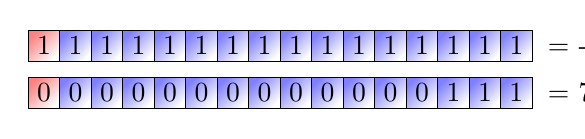
\begin{tikzpicture}[]
\shadedraw [top color=red!50,shading angle=45] (0,0) rectangle +(0.4,0.4);
\node at (0.2,0.2) {0};
\foreach \x in {0.4, 0.8, ..., 6.4}
   \shadedraw [top color=blue!50,shading angle=45] (\x,0) rectangle +(0.4,0.4);
\foreach \x in {0.6, 1.0, ..., 5.0}
   \node at (\x, 0.2){0};
\foreach \x in {5.4, 5.8, 6.2}
   \node at (\x, 0.2){1};   
\node at (6.6, 0.2){\rlap{= 7}};

\shadedraw [top color=red!50, shading angle=45] (0,0.6) rectangle +(0.4,0.4);
\foreach \x in {0.4, 0.8, ..., 6.4}
   \shadedraw [top color=blue!50, shading angle=45] (\x,0.6) rectangle +(0.4,0.4);
\foreach \x in {0.2, 0.6, ..., 6.6}
   \node at (\x, 0.8){1};
\node at (6.6, 0.8){\rlap{= -1}};
\end{tikzpicture}
\end{center}
(for more information see \kt{\tt <limits.h>})
\end{frame}


\begin{frame}
\frametitle{Integer Types(2)}
\begin{itemize}
\item Two main subtypes \emph{signed} and \emph{unsigned}. Signed types use a sign bit.
\item For signed types we, usually, have:
\begin{itemize}
\item minimum value: $-2^{\textrm{size}-1}$
\item maximum value: $2^{\textrm{size}-1}-1$
\end{itemize}
\item For unsigned types we have:
\begin{itemize}
\item minimum value: $0$
\item maximum value: $2^{\textrm{size}}-1$
\end{itemize}
\item \kw{\tt short} is often used to conserve memory.
\item \kw{\tt int} represents the \emph{native} CPU integer type so is used for speed. (If in doubt use \kw{\tt int}).
\item \kw{\tt long} and \kw{\tt long long} are used to maintain accuracy.
\end{itemize}
\end{frame}

\begin{frame}
\frametitle{Integer Arithmetic}

\begin{block}{Base Operators}
The four usual operators are defined $+$, $-$, {\tt *} and $/$.
\end{block}

\begin{block}{Ring arithmetic}
Division is not always the reverse of multiplication:\\
{\tt 1/2=0,  0*2=0.}\\
Also, any result of a computation must lie within the ring, any number outside the range of the current data type will ``wrap'' around. (i.e. 11am + 3 hours gives 2pm).
\end{block}

\begin{block}{Remainder Operator}
The remainder operator {\tt\%} is unique to integer types, it acts as expected:
{\tt7\%2 = 1}.
\end{block}
\end{frame}

\subsection{Floating Point}
\begin{frame}
\frametitle{Floating Point Numbers (IEEE 754 Standard)}
On my machine, a \kw{\tt float} (single precision) looks like:\\
\begin{center}
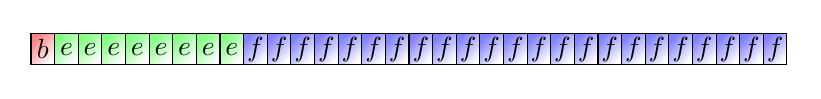
\begin{tikzpicture}[]
\shadedraw [top color=red!50,shading angle=45] (0,0) rectangle +(0.3,0.4);
\node at (0.15,0.2) {$b$};
\foreach \x in {0.3, 0.6, ..., 2.7}
   \shadedraw [top color=green!50,shading angle=45] (\x,0) rectangle +(0.3,0.4);

\foreach \x in {0.45, 0.75, ..., 2.85}
   \node at (\x,0.2) {$e$};
   
\foreach \x in {2.7, 3.0, ..., 9.6}
   \shadedraw [top color=blue!50,shading angle=45] (\x,0) rectangle +(0.3,0.4);
   
\foreach \x in {2.85, 3.15, ..., 9.45}   
   \node at (\x,0.2) {$f$};
\end{tikzpicture}
\end{center}
It consists of three parts, the \textcolor{red}{\emph{sign bit}$(b)$}, the \textcolor{green}{\emph{biased exponent}$(e)$} and the \textcolor{blue}{\emph{fraction}$(f)$}.
We break down a number $x$:
$$x^{\textrm{float}} = \textcolor{red}{(-1)^b} \times 
\textcolor{green}{2^{e-127}} \times \textcolor{blue}{\left(1+f\times2^{-23}\right)},
\begin{array}{c}
0 < e < 255\\0 \leq f \leq 2^{23}-1
\end{array},$$
We have three special numbers, {\tt -Inf} ($-\infty$), {\tt Inf} ($\infty$) and {\tt NaN} (Not a Number).

For \kw{\tt double} (double precision) we have:
$$x^{\textrm{double}} = (-1)^b\times 2^{e-1023}\times\left(1+f\times2^{-52}\right),
\begin{array}{c}
0 < e < 2047\\0 \leq f \leq 2^{52}-1
\end{array}.$$
\end{frame}

\begin{frame}
\frametitle{Floating Point}
\begin{block}{Base Operators}
As with integers, we have $+$, $-$, {\tt *} and $/$.
\end{block}

\begin{block}{Floating point code}
\begin{itemize}
\item It looks like integer code but with a decimal point suffix.
\item Scientific notation is achieved with {\tt e}:\\
{\tt \kw{double} speedofLight = 2.997e8;} ($2.997 \times 10^8$)
\end{itemize}
\end{block}

\begin{block}{Float Arithmetic}
\begin{itemize}
\item Division is not always the reverse of multiplication.
\item Operators may not be commutative!
$$ A + B + C \neq A + C + B \qquad \mathrm{(sometimes)}$$
\end{itemize}
\end{block}
\end{frame}

\subsection{Mathematical Functions}
\begin{frame}
\frametitle{More Mathematical Functions in \kt{\tt <math.h>}}
\begin{itemize}
\item Maths functions come with the \emph{ANSI Standard C Library}, which contains many maths functions. To use them we need a:
{\tt \kw{\#include} \kt{<math.h>}}
\item Here some example functions:
\begin{tabular}{l l l l}
\tt sin(x)&\tt asin(x) & \tt sinh(x) & \tt exp(x)\\
\tt cos(x)&\tt acos(x) & \tt cosh(x) & \tt log(x)\\
\tt tan(x)&\tt atan(x) & \tt tanh(x) & \tt log10(x)\\
\tt sqrt(x)&\tt atan2(x,y)&\tt pow(x,y) & \tt fabs(x)
\end{tabular}\\
\vspace{1ex}
(all the trigonometric functions use radians!)
\end{itemize}
\end{frame}

\begin{frame}
\frametitle{The {\tt pow(x, y)} function (declared in \kt{\tt <math.h>})}
\begin{block}{Exponentiation}
There is no exponentiation operator (e.g. $\wedge$, {\tt **}) in C. Instead we have the following:
$$x^y = \mathrm{\tt pow(x,y)}$$
This assumes $x$ and $y$ are of type \kw{\tt double}.
\end{block}

\begin{alertblock}{Beware}
The {\tt pow} function is often implemented as:
\begin{center}{\tt exp(y*ln(x))}\end{center}
For whole integer powers (i.e. $x^2$), one should perform the multiplication explicitly ({\tt x*x}).
\end{alertblock}
\end{frame}

\subsection{C Shorthand}
\begin{frame}[fragile]
\frametitle{Cryptic C}
There are shortcuts in the C language that allow for concise code.
\begin{enumerate}
\item Incrementing by 1: Pre-increment, and post-increment.\\
\begin{tabular}{l l}
\tt ++i& Increment {\tt i} by 1, then use it.\\
\tt i++& Use {\tt i}, then increment it by 1.
\end{tabular}
\item Increment by another variable.\\
\begin{tabular}{r l}
Normal code:&\tt sum = sum + v[i];\\
Terse code:&\tt sum += v[i];
\end{tabular}
\end{enumerate}
An example:\\
\begin{semiverbatim}
   \kw{for} (i=0; i < N; i++)
      sum += v[i];
\end{semiverbatim}
\end{frame}

\begin{frame}
\frametitle{More Shorthand}
\begin{tabular}{l l}
\tt --i;&decrement {\tt i} by 1.\\
\tt sum -= v[i];&means {\tt sum = sum - v[i];}\\
\tt sum *= v[i];&means {\tt sum = sum * v[i];}\\
\tt sum /= v[i];&means {\tt sum = sum / v[i];}\\
\tt sum \%= 2;&means {\tt sum = sum \% 2;}
\end{tabular}
Other operators can also be abbreviated this way.
\begin{exampleblock}{Inline {\tt if}}
The following code:
\begin{center}
\tt \kw{if} (r1 > r2) maxr = r1; \kw{else} maxr = r2;
\end{center}
can be abbreviated:
\begin{center}
\tt maxr = (r1 > r2) ? r1 : r2;
\end{center}
\end{exampleblock}
\end{frame}



\section{Control Flow Statements}
\subsection{Logical Expressions}
\begin{frame}
\frametitle{Simple Logical Expressions}
\texttt{\krr{7}\kl   \kw{while} (c <= high)}\\ 
\begin{itemize}
\item Are used to carry out branches ({\tt \kw{if}} statement) and loops (such as {\tt \kw{for}}, and {\tt \kw{while}}).
\item Evaluate to either \emph{true} (non-zero \kw{\tt int}) or \emph{false} (zero).
\end{itemize}

\begin{block}{Logical Operators}
\begin{center}
\begin{tabular}{l c l l}
\tt x &\tt>&\tt  y& is {\tt x} greater than {\tt y}?\\
\tt x &\tt>=&\tt y& is {\tt x} greater than or equal to {\tt y}?\\
\tt x &\tt<&\tt  y& is {\tt x} less than {\tt y}?\\
\tt x &\tt<=&\tt y& is {\tt x} less than or equal to {\tt y}?\\
\alert{\tt x }&\tt\alert{==}&\alert{\tt y}&\alert{is {\tt x} equal to {\tt y}?}\\
\tt x &\tt!=&\tt y& is {\tt x} different to {\tt y}?
\end{tabular}
\end{center}
\end{block}
\end{frame}

\begin{frame}
\frametitle{Compound Logical Expressions}
We can create compound logical expressions using the following operators:
\begin{itemize}
 \item {\tt ||} is a \emph{logical or}. {\tt le1 || le2} returns false if both {\tt le1} and {\tt le2} are false and true otherwise.
 \item {\tt \&\&} is a \emph{logical and}. {\tt le1 \&\& le2} returns true if and only if both {\tt le1} and {\tt le2} are true.
 \item {\tt !} is a \emph{logical not}. {\tt !le1} returns the opposite of {\tt le1}.
\end{itemize}
Here are two identical examples:
\begin{itemize}
\item \tt (x < 100) \&\& (x\%2 == 0)\\
\item \tt (x < 100) \&\& !(x\%2)
\end{itemize}
\end{frame}

\subsection{Control Statements}
\begin{frame}[fragile]
\frametitle{Flow Control - {\tt if}}
Executes block(s) of code depending on the evaluation of a logical expression.
\begin{block}{Simple {\tt if}}
\begin{center}{\tt \kw{if} (}\emph{logical expression}{\tt ) \{}\emph{statements}{\tt ;\}}\end{center}
\end{block}

\begin{block}{{\tt if}, {\tt else if}, {\tt else}}
\begin{semiverbatim}
   \kw{if} (\emph{logical expression})
      \{\emph{statements};\}
   \kw{else if} (\emph{logical expression})
      \{\emph{statements};\}
   \kw{else if} (\emph{logical expression})
      \{\emph{statements};\}
   \kw{else}
      \{\emph{statements};\}
\end{semiverbatim}
\end{block}
\end{frame}

\begin{frame}[fragile]
\frametitle{Flow Control - {\tt while}}
A \kw{\tt while} loop is used to repeatedly execute code as long as a logical expression is true.

\begin{block}{Structure}
\begin{semiverbatim}
   \kw{while} (\emph{logical expression})
      \{ \emph{statements} ;\}
\end{semiverbatim}
\end{block}
\begin{itemize}
\item If \emph{logical expression} is false, then the \emph{statements} are never executed.
\end{itemize}
\end{frame}

\begin{frame}[fragile]
\frametitle{Flow Control - {\tt do \{\} while ()}}
We place the \emph{logical expression} after the \emph{statements} giving us:
\begin{block}{Structure}
\begin{semiverbatim}
   \kw{do} \{\emph{statements};\}
   \kw{while} (\emph{logical expression})
\end{semiverbatim}
\end{block}
\begin{itemize}
\item The \emph{statements} are executed at least once.
\end{itemize}
\begin{exampleblock}{{\tt do while} or {\tt while}?}
Generally I prefer {\tt \kw{while}} over {\tt \kw{do while}}, as it forces me to initialise variables properly.
\end{exampleblock}
\end{frame}

\begin{frame}[fragile]
\frametitle{Flow Control - {\tt for} loop}
\begin{block}{}
\begin{semiverbatim}
   \kw{for} ( \emph{start expression} ;
         \emph{logical expression} ;
         \emph{step expression})
         \{ \emph{statements} ;\}
\end{semiverbatim}
\end{block}
\begin{itemize}
\item Print out ten numbers:
\begin{semiverbatim}
   \tt\kw{for} (x=0; x < 10; x = x + 1)
      printf(\kt{"x = %d\\n"}, x);
\end{semiverbatim}
\item Keep looping indefinitely (printing out dots)
\begin{semiverbatim}
   \kw{for} (;;) printf(\kt{"."});
\end{semiverbatim}
\end{itemize}
\end{frame}

\begin{frame}[fragile]
\frametitle{Flow Control - \tt switch - case}
We can selectively execute code based on a value, using the following:
\begin{block}{}
\begin{semiverbatim}
   \kw{switch} (\emph{integer\_statement}) \{
   \kw{case} \emph{integer\_value1}: \emph{statements1}; \kw{break};
   \kw{case} \emph{integer\_value2}: \emph{statements2}; \kw{break};
   \kw{case} \emph{integer\_value3}:
   \kw{case} \emph{integer\_value4}: \emph{statements3}; \kw{break};   
   \kw{default}: \emph{statements4}; \kw{break};\}
\end{semiverbatim}
\end{block}
\begin{itemize}
\item Execution starts at either one of the \kw{\tt case}'s or at \kw{\tt default}.
\item Execution stops at the end {\tt\}} or at \kw{\tt break}.
\item \kw{\tt case}, \kw{\tt default} and \kw{\tt break} are optional.
\end{itemize}
\end{frame}

\begin{frame}{Some Loop Control Features}
Execution of code inside a loop (\kw{\tt do}, \kw{\tt while}, \kw{\tt for})
can be manipulated by the following statements.
\begin{block}{\tt break;}
Break out of the current loop. Any statements in the loop following the \kw{\tt break} are ignored and the loop condition automatically evaluates to false, ending the loop.
\end{block}
\begin{block}{\tt continue;}
Jump to the end of the current loop (effectively ignoring everything below the \kw{\tt continue} statement. Whether or not the loop continues executing depends on the loop condition.
\end{block}
\end{frame}

\section{Interacting with the Console}
\subsection{printf}
\begin{frame}
\frametitle{{\tt printf} - declared in \kt{\tt <stdio.h>}}
As seen in the examples, the {\tt printf} function can be used to print out variables. The function \emph{prototype} takes the form:
\begin{center}
{\tt \alert<4>{\kw{int}} printf(\alert<2>{\kw{char} * formatString}, \alert<3>{...})}
\end{center}
\begin{block}<2>{{\tt formatString}}
The first argument of {\tt printf} is the \emph{format string}, this specifies how many variables need printing out, how they are to be printed, and in what order.
\end{block}
\begin{block}<3>{{\tt ...}}
This is C shorthand for \emph{variable number of arguments}.
\end{block}

\begin{block}<4>{Return value: {\tt int}}
{\tt printf} returns the number of characters printed.
\end{block}
\end{frame}

\begin{frame}
\frametitle{{\tt printf} - declared in \kt{\tt <stdio.h>}}
We call {\tt printf} as follows:
\begin{center}
\tt printf(formatString, var1, var2, $\ldots$, varN);
\end{center}
where,
\begin{block}{\tt formatString}
The format string tells {\tt printf} how many variables need printing. A format string can contain \emph{format specifiers}, these tell {\tt printf} exactly how to print out each variable, some examples:
\begin{tabular}{l l}
\tt\kt{"\%6d"} & print out an integer (6 characters wide).\\
\tt\kt{"\%g"} & print out a floating point number.
\end{tabular}
\end{block}
\begin{block}{\tt var1, ...}
{\tt printf} accepts a variable list of arguments, which can be of different type. Care must be taken to match {\tt formatString} with the variables.
\end{block}
\end{frame}

\begin{frame}
\frametitle{Special Characters}
\begin{itemize}
\item The backslash {\tt $\backslash$} character in C has a special meaning, it is known as the \emph{escape character}.
\item We combine the escape character with other characters, to form an \emph{escape sequence}, here are some examples:
\begin{center}
\begin{tabular}{l r}
\begin{tabular}{r l}
{\tt $\backslash$n} & New line\\
{\tt $\backslash$t} & Tab\\
{\tt $\backslash$b} & Backspace\\
{\tt $\backslash$r} & Carriage return\\
{\tt $\backslash$a} & Bell
\end{tabular}&
\begin{tabular}{r l}
{\tt $\backslash$f} & Form feed (new page)\\
{\tt $\backslash\backslash$} & $\backslash$\\
{\tt $\backslash$"} & "\\
{\tt $\backslash$'} & '
\end{tabular}
\end{tabular}
\end{center}
\end{itemize}
\end{frame}

\subsection{scanf}
\begin{frame}{{\tt scanf()} - Reading Data from Standard Input}
For two variables {\tt A} and {\tt B}, both of type \kw{\tt double}, we use:
\begin{center}
\tt scanf(\kt{"\%lf \%lf"}, \&A, \&B);
\end{center}
\begin{itemize}
\item where the {\tt\%} represent \emph{format specifiers}
\begin{block}{Format Specifiers}
Consist of a {\tt\%}, a numerical width specification and a field code:
\resizebox{\textwidth}{!}{
\begin{tabular}{c c}
\begin{tabular}{l l}
\tt d& \kw{\tt int}\\
\tt u& \kw{\tt unsigned int}\\
\tt f& \kw{\tt float} (fixed form)\\
\tt e& \kw{\tt float} (exponential form)
\end{tabular}&
\begin{tabular}{l l}
\tt g & \kw{\tt float} (general form)\\
\tt lf & \kw{\tt double} (fixed form)\\
\tt le & \kw{\tt double} (exponential form)\\
\tt lg & \kw{\tt double} (general form)
\end{tabular}
\end{tabular}}
\end{block}
\item and the {\tt\&} represents the \emph{address} of the variable in memory. This is known as a \emph{pointer reference operator}.
\end{itemize}
\end{frame}

\begin{frame}
\frametitle{Why the {\tt \&A} in {\tt scanf()}?}
\begin{itemize}
\item Functions in C can return only one value.
\item Sometimes we want more than one value to change.
\item If we tell {\tt scanf} \emph{where} the variables are in memory,
{\tt scanf} can change them itself.
\end{itemize}

\begin{alertblock}{}
The ability to manipulate memory directly is what makes C so powerful.
(and potentially dangerous).
\end{alertblock}
\end{frame}

\subsection{Touching on Pointers}
\begin{frame}[fragile]
\frametitle{Pointers}
A \emph{pointer} is a variable that stores a memory location, they are declared as follows:
\begin{center}
\tt \kw{double} * ptrA;
\end{center}

\begin{block}{{\tt \&} - Pointer reference operator}
Returns the memory address (pointer to) of a variable.
\begin{semiverbatim}
   \kw{double} * ptrA = \&A;   \kc{// ptrA points to A}
\end{semiverbatim}
\end{block}

\begin{block}{{\tt *} - Pointer de-reference operator}
Converts a memory address to a variable:
\begin{semiverbatim}
   * ptrA  = 1.234;      \kc{// A is now 1.234}
\end{semiverbatim}
\end{block}
\end{frame}



\section{Functions}

\subsection{Defining Functions}
\begin{frame}
\frametitle{Defining Functions}
The C language only provides essential functionality, meaning a lot of functions need to be written yourself. Here are a few general rules for functions:

\begin{itemize}
\item Functions cannot define other functions within them.
\item An optional single value can be returned.
\item All arguments to a functions are passed by value and remain unaffected by the function.
\item Passing pointers to functions allows them to ``return'' multiple variables.
\end{itemize}
\end{frame}

\begin{frame}[fragile]
\frametitle{Declarations vs Definitions}
\begin{block}{Function Declarations}
These tell the compiler about the \emph{existence} of a function, which then
allows us to call it. A declaration ends with a {\tt ;}.
\begin{semiverbatim}
\kw{int} quad_roots (\kw{double} A, \kw{double} B, \kw{double} C,
                \kw{double} * r1, \kw{double} * r2);
\end{semiverbatim}
\end{block}

\begin{block}{Function Definitions}
The code making up the function is supplied to the compiler. A function can only be defined once. A definition contains braces {\tt \{} and {\tt \}}:
\begin{semiverbatim}
\kw{int} quad_roots (\kw{double} A, \kw{double} B, \kw{double} C,
                \kw{double} * r1, \kw{double} * r2)
\{...\}
\end{semiverbatim}
\end{block}
\end{frame}

\begin{frame}
\frametitle{Functions with Variable Number of Arguments}
Sometimes we don't know in advance how many arguments (or what type) a function needs, so C allows functions to have an unknown number of arguments. Two examples we've seen so far are {\tt printf} and {\tt scanf}.

\begin{itemize}
\item The first parameter must be of a normal type (i.e. \kw{\tt int}).
\item Three dots ({\tt ...}) are used for the last parameter.
\end{itemize}
\begin{center}
{\tt \kw{int} printf(\kw{char} * formatString, ...)}
\end{center}
\begin{block}{Handling variable arguments}
Variable arguments are manipulated using {\tt va\_start()}, {\tt va\_arg()},
and {\tt va\_end()}. These are found in \kt{\tt <stdarg.h>}.
\end{block}

\begin{alertblock}{}
Having just introduced these, I'm going to ask you {\bf not} to use them! Arrays are almost always more appropriate to use.
\end{alertblock}
\end{frame}

\subsection{Using Functions}
\begin{frame}
\frametitle{An Example: Quadratic Equation Solver}
As a worked example we write a function to solve the quadratic equation:
$$ A x^2 + B x + C=0 \qquad A,B,C\in\mathbb{R}$$
Our quadratic solver will:
\begin{itemize}
\item Take the three doubles {\tt A}, {\tt B} and {\tt C} as arguments.
\item Solve the quadratic and return an \kw{\tt int} signifying to the caller the type of answer available:
\begin{tabular}{l l}
-1&{\tt A} = 0, we have a linear equation.\\
0&There are two distinct real roots.\\
1&We have a pair of complex conjugate roots.\\
2&Both roots are real and identical.
\end{tabular}
\end{itemize}
\end{frame}

\begin{frame}[fragile]
\frametitle{The Code}
One possible function prototype is:
\begin{semiverbatim}
\kw{int} quad_roots (\kw{double} A, \kw{double} B, \kw{double} C,
                \kw{double} * r1, \kw{double} * r2);
\end{semiverbatim}
\begin{itemize}
\item The variables {\tt A}, {\tt B} and {\tt C} are unchanged by {\tt quad\_roots}.
\item We need to return two doubles (the roots of the equation), thus we take in pointers {\tt \kw{double} *r1} and {\tt \kw{double} *r2}.
\item C90 does not allow for complex number types (C99 does support them), so we have to think a little bit about the complex number case.
\end{itemize}
\end{frame}

\begin{frame}[fragile]
\frametitle{Code Snippet for Calling {\tt quad\_roots}}
\begin{semiverbatim}
...
\kw{int} main()
\{
   \kw{double} A, B, C, root1, root2;
   \kw{int} quad_case;   
   ...   
   quad\_case = quad\_roots(A, B, C, \&root1,
                          \&root2);
                          
   \kw{switch}(quad\_case)
   \{
   \kw{case} -1: \emph{linear equation}
\end{semiverbatim}
\end{frame}

\begin{frame}[fragile]
\frametitle{Code Snippet for {\tt quad\_roots}}
\begin{semiverbatim}
\kw{int} quad\_roots(\kw{double} A, \kw{double} B, \kw{double} C,
               \kw{double} * r1, \kw{double} *r2)
\{
   \kw{double} d;
   
   \kc{/* linear case */}
   if (A == 0.0)
   \{
      *r1 = -C/B;
      \kw{return} -1;
   \}
          
   \kc{/* compute the discriminant */}
   d = B*B-4.0*A*C;
\end{semiverbatim}
\end{frame}

\subsection{Structuring Functions}
\begin{frame}[fragile]
\frametitle{The Stack}
Let's consider this example function.
\begin{columns}
\begin{column}{5cm}
\begin{semiverbatim}
\kw{int} hasRealRoots(\alert<2>{\kw{double} A},
       \alert<2>{\kw{double} B, \kw{double} C})
\{
   \alert<3>{\kw{double} d} = B*B-4.0*A*C;
   \kw{if} (d < 0) \alert<4>{\kw{return}} 0;
   \alert<4>{\kw{return}} 1;
\}
\end{semiverbatim}
\end{column}
\begin{column}{5cm}
\begin{itemize}
\alert<2>{\item We need space to hold a copy of {\tt A}, {\tt B} and {\tt C}.} 
\alert<3>{\item We need space to store our computed {\tt d}.}
\alert<4>{\item When we've finished, we need to get back to the calling function.}
\end{itemize}
\end{column}
\end{columns}
\vspace{0.1in}
\begin{block}<5>{}
\begin{center}
\alert<5>{This is achieved by using a \emph{stack}.}
\end{center}
\end{block}
\end{frame}

\begin{frame}
\frametitle{The Stack - Rough Sketch (Stack Frames)}
\begin{columns}
\begin{column}{5cm}
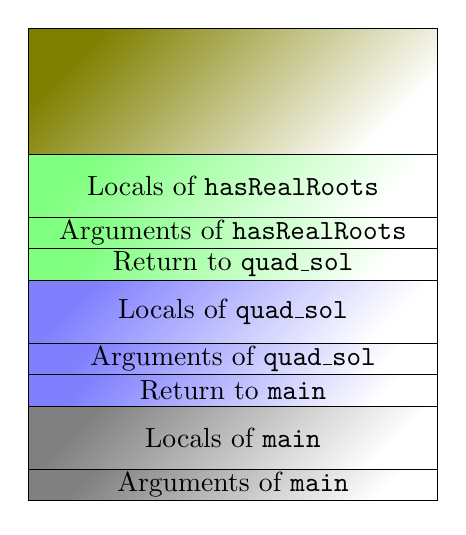
\begin{tikzpicture}[]
\shadedraw [shading angle=45] (0,0) rectangle +(5.2,0.4);
\node at (2.6,0.2) {Arguments of \tt main};
\shadedraw [shading angle=45] (0,0.4) rectangle +(5.2,0.8);
\node at (2.6,0.8) {Locals of \tt main};
\shadedraw [top color=blue!50,shading angle=45] (0,1.2) rectangle +(5.2,0.4);
\node at (2.6,1.4) {Return to \tt main};
\shadedraw [top color=blue!50,shading angle=45] (0,1.6) rectangle +(5.2,0.4);
\node at (2.6,1.8) {Arguments of \tt quad\_sol};
\shadedraw [top color=blue!50,shading angle=45] (0,2.0) rectangle +(5.2,0.8);
\node at (2.6,2.4) {Locals of \tt quad\_sol};
\shadedraw [top color=green!50,shading angle=45] (0,2.8) rectangle +(5.2,0.4);
\node at (2.6,3.0) {Return to \tt quad\_sol};
\shadedraw [top color=green!50,shading angle=45] (0,3.2) rectangle +(5.2,0.4);
\node at (2.6,3.4) {Arguments of \tt hasRealRoots};
\shadedraw [top color=green!50,shading angle=45] (0,3.6) rectangle +(5.2,0.8);
\node at (2.6,4.0) {Locals of \tt hasRealRoots};
\shadedraw [top color=green!50!red,shading angle=45] (0,4.4) rectangle +(5.2,1.6);
\end{tikzpicture}
\end{column}
\begin{column}{6cm}
\begin{itemize}
\item Consider the case where we have {\tt main}, which calls \textcolor{blue}{\tt quad\_sol}, which in turn calls \textcolor{green}{\tt hasRealRoots}.
\item We add and remove items from the stack as the program executes.
\item Adding/removing items from the stack takes very little time.
\item The stack is fixed in size, if we go over the top (``smash the stack'')
, our program crashes.
\end{itemize}
\end{column}
\end{columns}
\end{frame}

\begin{frame}
\frametitle{Recursive Functions}
As C uses a stack by default when calling functions, we are able to write functions that call themselves. These are called \emph{recursive functions}.

\begin{block}{An Example: Computing the Factorial}
$$n! = \prod_{i=1}^n i,  \quad 0! = 1, \qquad n\in\mathbb{N}.$$
Lends itself to be coded up as a recursive function.
\end{block}

\begin{block}{A Tougher Example: Fibonacci Numbers}
$$ F_n = F_{n-1} + F_{n-2}, \qquad F_0 = F_1 = 1.$$
A na\"ive implementation of this will kill the stack, and take a very long time to execute.
\end{block}
\end{frame}

\begin{frame}[fragile]
\frametitle{Computing the Factorial}
\begin{semiverbatim}
\kr\kl\kw{\#include} \kt{<stdio.h>}
\kl
\kl\kw{int} NFact(\kw{int} N)
\kl\{
\kl   \kw{if} (N>1) \kw{return} N*NFact(N-1);
\kl   \kw{return} 1;
\kl\}
\kl
\kl\kw{int} main()
\kl\{
\kl   \kw{int} n;
\kl   printf(\kt{"Enter n:"});
\kl   scanf(\kt{"%d"}, &n);
\kl   printf(\kt{"%d! = %d\\n"}, n, NFact(n));
\kl   \kw{return} 0;
\kl\}
\end{semiverbatim}
\end{frame}

\begin{frame}[fragile]
\frametitle{Computing Fibonacci Numbers}
\begin{columns}
\begin{column}{6cm}
\begin{alertblock}{}
\begin{semiverbatim}
\kw{int} BadFib(\kw{int} N)
\{
   \kw{if} (N < 2) \kw{return} 1;
   \kw{return} (BadFib(N-1) +
           BadFib(N-2));
\}
\end{semiverbatim}
\end{alertblock}
\end{column}
\begin{column}{3cm}
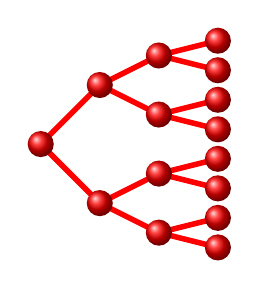
\begin{tikzpicture}[scale=0.75]
\tikzstyle{every node}=[ball color=red,circle,text=white]
\tikzstyle{edge from parent}=[draw,dashed,thick,red]
\draw[line width=2pt,color=red] (0,0) -- (1.0,1.0);
\draw[line width=2pt,color=red] (0,0) -- (1.0,-1.0);
\draw[line width=2pt,color=red] (1.0,1.0) -- (2.0,1.5);
\draw[line width=2pt,color=red] (1.0,1.0) -- (2.0,0.5);
\draw[line width=2pt,color=red] (1.0,-1.0) -- (2.0,-0.5);
\draw[line width=2pt,color=red] (1.0,-1.0) -- (2.0,-1.5);
\draw[line width=2pt,color=red] (2.0,1.5) -- (3.0,1.75);
\draw[line width=2pt,color=red] (2.0,1.5) -- (3.0,1.25);
\draw[line width=2pt,color=red] (2.0,0.5) -- (3.0,0.75);
\draw[line width=2pt,color=red] (2.0,0.5) -- (3.0,0.25);
\draw[line width=2pt,color=red] (2.0,-0.5) -- (3.0,-0.25);
\draw[line width=2pt,color=red] (2.0,-0.5) -- (3.0,-0.75);
\draw[line width=2pt,color=red] (2.0,-1.5) -- (3.0,-1.75);
\draw[line width=2pt,color=red] (2.0,-1.5) -- (3.0,-1.25);
\node at (0,0) {};
\node at (1.0, 1.0) {};
\node at (1.0, -1.0) {};
\node at (2.0, 1.5) {};
\node at (2.0, 0.5) {};
\node at (2.0, -0.5) {};
\node at (2.0, -1.5) {};
\node at (3.0, 1.75) {};
\node at (3.0, 1.25) {};
\node at (3.0, 0.75) {};
\node at (3.0, 0.25) {};
\node at (3.0, -0.75) {};
\node at (3.0, -0.25) {};
\node at (3.0, -1.75) {};
\node at (3.0, -1.25) {};
\end{tikzpicture}
\end{column}
\end{columns}

\begin{columns}
\begin{column}{7cm}
\begin{exampleblock}{}
\begin{semiverbatim}
\kw{int} utilf(\kw{int} a, \kw{int} b, \kw{int} n)
\{
   \kw{if}(n < 1) \kw{return} b;
   \kw{return} utilf(b, a+b, n-1);
\}
\kw{int} GoodFib(\kw{int} n)
\{
   \kw{return} utilf(0, 1, n);
\}
\end{semiverbatim}
\end{exampleblock}
\end{column}
\begin{column}{3cm}
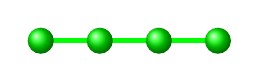
\begin{tikzpicture}[scale=0.75]
\tikzstyle{every node}=[ball color=green,circle,text=white]
\tikzstyle{edge from parent}=[draw,dashed,thick,green]
\draw[line width=2pt,color=green] (0,0) -- (1.0,0.0) -- (2.0, 0.0) -- (3.0, 0.0);
\node at (0,0) {};
\node at (1,0) {};
\node at (2,0) {};
\node at (3,0) {};
\end{tikzpicture}
\end{column}
\end{columns}
\end{frame}

\subsection{Code Structure}
\begin{frame}
\frametitle{Imperative versus Functional Programming}
Two programming techniques are popular in C:
\begin{alertblock}{Imperative}
\begin{itemize}
\item Very long functions.
\item Lots of global variables.
\item Very few function calls.
\end{itemize}
\end{alertblock}

\begin{exampleblock}{Functional}
\begin{itemize}
\item Lots of small functions.
\item Each function has a clearly defined r\^ole.
\item Global variables avoided as much as possible.
\end{itemize}
\end{exampleblock}
I would encourage leaning towards the latter, a good program will contain traits from both styles.
\end{frame}




\subsection{Functions - Summary}
\begin{frame}
\frametitle{Functions - Summary}
\begin{itemize}
\item Functions need to be declared before they are used. This is often done in \emph{header files}.
\item Up to one value can be returned from a function using the \kw{\tt return} statement.
\item A variable {\tt var} can be changed by a function if we pass the pointer
{\tt \&var}.
\item Pointers are declared using {\tt type * variable;}
\end{itemize}
\end{frame}

\section{Arrays}
\subsection{Data Arrays}
\begin{frame}
\frametitle{Arrays}
\begin{itemize}
\item These are blocks of data, all of the same type. Each element is indexed
using the array index operator:\\
e.g. {\tt myArray[index]} or {\tt primes[3]}.
\item Arrays are declared with types and sizes:\\
e.g. {\tt \kw{double} xVector[3];}
\item Arrays can be initialised:\\
e.g. {\tt \kw{int} primes[6] = \{2, 3, 5, 7, 11, 13\};}
\item All the elements of an array can be initialised to the \emph{same} value:
e.g. {\tt \kw{double} lotsOfDoubles[100] = \{0.0\};}
\item \bf Arrays in C are indexed from 0!
\end{itemize}
\end{frame}

\begin{frame}[fragile]
\frametitle{Accessing Array Elements}
\begin{alertblock}{}
\begin{center}
\bf Arrays in C are indexed from 0!
\end{center}
\end{alertblock}
\begin{semiverbatim}
\kw{\#include} \kt{<stdio.h>}

\kw{int} main()
\{
   \kw{int} primes[6] = \{2, 3, 5, 7, 11, 13\};

   printf(\kt{"first prime = \%d\\n"}, primes[0]);
   printf(\kt{"next prime = \%d\\n"}, primes[1]);
   
   \kw{return} 0;   
\}
\end{semiverbatim}
\end{frame}

\subsection{A Little More on Pointers}
\begin{frame}
\frametitle{A little more on pointers}
\begin{block}{Reminder}
\begin{itemize}
\item Declared using: {\tt type * ptrVar;}
\item Variable to pointer (pointer \emph{referencing}): {\tt ptrA = \&A;}
\item Pointer to variable (pointer \emph{de-referencing}):\\ {\tt *ptrA = newVar;}
\end{itemize}
\end{block}
\begin{exampleblock}{In addition}
Pointers are memory addresses, and as such allow arithmetic!
\end{exampleblock}
\end{frame}

\begin{frame}[fragile]
\frametitle{Pointer Arithmetic}
\begin{itemize}
\item Different data types in C are different sizes.
\item Pointers are usually declared with a type (i.e. {\tt \kw{int} *},
{\tt \kw{float} *}, {\tt \kw{double} *}).

\begin{alertblock}{Relation to Arrays}
Given the array {\tt myArray} and an integer {\tt index}, the following is true:
\begin{center}
\tt myArray[index] = *(myArray + index)
\end{center}
\end{alertblock}

\item And this is the reason array indices start at 0...
\end{itemize}

\end{frame}

\section{Debugging}
\subsection{Debugging Techniques}
\begin{frame}
\frametitle{Debugging}
\begin{itemize}
\item Once you've designed, typed up and successfully compiled your program, the difficult part begins! Debugging!
\item Problems in the code are usually either easy to locate or stubbornly elusive.
\end{itemize}

\begin{exampleblock}{Easier Problems}
\begin{itemize}
\item Program crash/fault at the same point every run.
\end{itemize}
\end{exampleblock}

\begin{alertblock}{Nastier Problems}
\begin{itemize}
\item Numerical output differs to what is expected.
\item Program crashes seemingly randomly.
\end{itemize}
\end{alertblock}
\end{frame}

\begin{frame}
\frametitle{Debugging Techniques}
\begin{small}
In increasing order of difficulty:
\begin{block}{Create Verbose Output}
\begin{itemize}
\item A few strategically placed {\tt printf} statements can prove to be helpful, but they are human readable:
\begin{itemize}
\item too few and you miss the problem,
\item too many and they rapidly become useless.
\end{itemize}
\item Straightforward to implement (and to comment out).
\end{itemize}
\end{block}

\begin{block}{Code Defensively}
\begin{itemize}
\item Consider specialised test cases.
\item Write code to test intermediate results.
\item Use the {\tt assert} macro.
\end{itemize}
\end{block}

\begin{block}{Use a Debugger}
For those non-trivial problems.
\end{block}
\end{small}
\end{frame}

\subsection{Assertion Checking}
\begin{frame}
\frametitle{Assertion Checking}
In the header \kt{\tt <assert.h>}, the macro {\tt assert} is defined. It has the following syntax:\\
\begin{center}
\tt assert(\emph{logical\_expression});
\end{center}
If \emph{logical\_expression} evaluates to false (zero) then:
\begin{itemize}
\item Program execution stops immediately.
\item An error message is sent to \emph{stderr} (the console) stating the line number where the assertion failed.
\end{itemize} 
\begin{block}{}
{\tt assert( a != 0); \kc{/* a should never be zero */}}
\end{block}
\begin{exampleblock}{Switching it off}
Placing {\tt \kw{\#define} NDEBUG} before all the \mbox{\tt \kw{\#include} \kt{<assert.h>}}
statements de-activates assertion checking.
\end{exampleblock}
\end{frame}

\begin{frame}[fragile]
\frametitle{Assertion Checking - An Example}
\vspace{-0.2in}
\begin{semiverbatim}
\scriptsize
\kr\kl\kw{\#include} \kt{<stdio.h>}
\kl\kw{\#include} \kt{<assert.h>}
\kl\kc{/* the sqrt function is much better than this... */}
\kl\kw{double} squareRoot(\kw{double} N)
\kl\{
\kl   \kw{double} x = 1.0;
\kl   \kw{int} loop;
\kl   \kc{/* negative numbers are not allowed! */}
\kl   assert(N >= 0.0);
\kl   \kw{if} (N == 0.0) \kw{return} 0.0;
\kl   \kw{for} (loop = 0; loop < 10; loop++)
\kl      x = (x*x+N)/(2.0*x);
\kl   \kw{return} x;
\kl\}
\kl
\kl\kw{int} main()
\kl\{
\kl   \kw{double} square;
\kl   printf(\kt{"Enter a non-negative number:"});
\kl   scanf(\kt{"\%lg"}, \&square);
\kl   \kc{/* SHOULD HAVE: if (x < 0.0) ...        */}
\kl   printf(\kt{"Square root = \%g\\n"}, squareRoot(square));
\kl   \kw{return} 0;
\kl\}
\end{semiverbatim}
\end{frame}

\subsection{Using a Debugger}
\begin{frame}
\frametitle{Using a Debugger}
\begin{itemize}
\item Two good debuggers are {\tt gdb} (GNU debugger) and Microsoft's Visual Studio debugger.
\item Programs need to be compiled with debug information.
\item Running a program straight through a debugger will show you the line of code that crashed it (if it crashes).
\end{itemize}

\begin{exampleblock}{Interactive Analysis of Running Code}
\begin{itemize}
\item Program execution can be paused at \emph{breakpoints}.
\item Functions can be \emph{stepped into}, \emph{stepped over}, or
\emph{stepped out from}.
\item Variables/arrays can be \emph{watched}.
\end{itemize}
\end{exampleblock}

\begin{alertblock}{}
Debuggers are very tricky to use at first, but can help isolate some very subtle problems.
\end{alertblock}
\end{frame}

\subsection{Compile-time Logic}
\begin{frame}[fragile]
\frametitle{The C Preprocessor - Conditional Compilation}
We have already seen the {\tt \kw{\#include}} statement. Conditional statements are also possible:
\vspace{-0.2in}
\begin{semiverbatim}
\small
\kr\kl\kw{\#include} \kt{<stdio.h>}
\kl
\kl\kw{int} main()
\kl\{
\kl\kw{\#ifdef} NDEBUG
\kl   printf(\kt{"Assertions DISABLED\\n"});
\kl\kw{\#else}
\kl   printf(\kt{"Assertions ENABLED\\n"});
\kl\kw{\#endif}
\kl   \kw{return} 0;
\kl\}
\end{semiverbatim}
\begin{alertblock}{}
This logic is performed at \emph{compile time}.
\end{alertblock}
\end{frame}


\section{Causes of Error}

\subsection{Maths}
\begin{frame}
\frametitle{Common Problems}
\begin{enumerate}
\item Misuse of Power!\\
$x^2$ should always be written {\tt x*x}, \emph{NOT} {\tt pow(x, 2.0)}.\\
$\sqrt{x}$ should be written {\tt sqrt(x)}, \emph{NOT} {\tt pow(x, 0.5)}.
\item Integer Division\\
Remember a fraction such as {\tt 1/3} is equal to zero. To get a floating point fraction, this should be rewritten {\tt 1.0/3.0}.
\end{enumerate}
\end{frame}

\subsection{Floating Point Numbers}
\begin{frame}
\frametitle{Floating Point Numbers (IEEE 754 Standard)}
\framesubtitle{(from the previous lecture)}
On my machine, a \kw{\tt float} (single precision) looks like:\\
\begin{center}
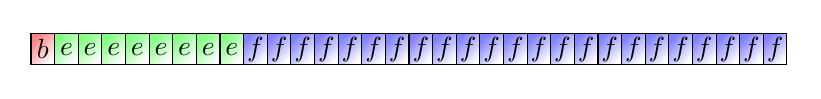
\begin{tikzpicture}[]
\shadedraw [top color=red!50,shading angle=45] (0,0) rectangle +(0.3,0.4);
\node at (0.15,0.2) {$b$};
\foreach \x in {0.3, 0.6, ..., 2.7}
   \shadedraw [top color=green!50,shading angle=45] (\x,0) rectangle +(0.3,0.4);

\foreach \x in {0.45, 0.75, ..., 2.85}
   \node at (\x,0.2) {$e$};
   
\foreach \x in {2.7, 3.0, ..., 9.6}
   \shadedraw [top color=blue!50,shading angle=45] (\x,0) rectangle +(0.3,0.4);
   
\foreach \x in {2.85, 3.15, ..., 9.45}   
   \node at (\x,0.2) {$f$};
\end{tikzpicture}
\end{center}
It consists of three parts, the \textcolor{red}{\emph{sign bit}$(b)$}, the \textcolor{green}{\emph{biased exponent}$(e)$} and the \textcolor{blue}{\emph{fraction}$(f)$}.
We break down a number $x$:
$$x^{\textrm{float}} = \textcolor{red}{(-1)^b} \times 
\textcolor{green}{2^{e-127}} \times \textcolor{blue}{\left(1+f\times2^{-23}\right)},
\begin{array}{c}
0 < e < 255\\0 \leq f \leq 2^{23}-1
\end{array},$$
We have three special numbers, {\tt -Inf} ($-\infty$), {\tt Inf} ($\infty$) and {\tt NaN} (Not a Number).

For \kw{\tt double} (double precision) we have:
$$x^{\textrm{double}} = (-1)^b\times 2^{e-1023}\times\left(1+f\times2^{-52}\right),
\begin{array}{c}
0 < e < 2047\\0 \leq f \leq 2^{52}-1
\end{array}.$$
\end{frame}

\begin{frame}
\frametitle{Floating Point Number Analysis}
In \kt{\tt <float.h>}, there are some useful quantities:
\resizebox{\textwidth}{!}{
\rowcolors[]{1}{blue!20}{blue!10}
\begin{tabular}{l l l}
\bf Quantity&\bf Float&\bf Double\\
Maximum Value&\tt FLT\_MAX&\tt DBL\_MAX\\
Minimum Value&\tt FLT\_MIN&\tt DBL\_MIN\\
Max Decimal Exponent&\tt FLT\_MAX\_10\_EXP&\tt DBL\_MAX\_10\_EXP\\
Min Decimal Exponent&\tt FLT\_MIN\_10\_EXP&\tt DBL\_MIN\_10\_EXP\\
$\epsilon$&\tt FLT\_EPSILON&\tt DBL\_EPSILON
\end{tabular}}

\begin{block}{Floating point $\epsilon$}
$\epsilon$ is the smallest (in magnitude) number such that:\\
\begin{center}
{\tt 1.0+$\epsilon$ != 1.0}
\end{center}
\end{block}
\end{frame}

\begin{frame}
\frametitle{Floating Point Accuracy}
\begin{itemize}
\item Some numbers can be represented in floating point exactly:
e.g. $2^i$, any integers that fit in the significand (mantissa).
\item Most numbers need to be approximated, e.g. $\sqrt{2}$, $\pi$.
\item One overlooked example is {\tt0.1}!
\item It is possible (though rare) to get exact answers from floating point arithmetic
\item Relative errors of $\approx10^{-15}$ for \kw{\tt double} and
$\approx10^{-6}$ for \kw{\tt float} are considered to be very good.
\item Multiplication and division generally preserve relative error (but can take us outside the floating point range).
\end{itemize}
\end{frame}

\begin{frame}
\frametitle{The Largest Source of Floating Point Errors}
Addition and subtraction are the largest contributors to floating point error.

\begin{alertblock}{The Golden Rule}
{\bf Do not subtract two very similar floating point numbers!}
\end{alertblock}

(This leads to ``\emph{catastrophic cancellation}''.)
\end{frame}

\subsection{Casting}
\begin{frame}[fragile]
\frametitle{Casting}
Casting can either be \emph{implicit} or \emph{explicit}.
\begin{block}{Implicit Casting}
Conversion where there is no ambiguity (i.e. to a ``bigger'' data type) can be done automatically:
\begin{semiverbatim}
\small\kw{double} x = 5; \kc{/* conversion from int to double */}
\kw{double} fEps = FLT\_EPSILON; \kc{/* float to double */}
\end{semiverbatim}
\end{block}

\begin{block}{Explicit Casting}
If we wish to force a type conversion we place the destination type in brackets before the source variable:
\begin{semiverbatim}
oldtype oldData = ...
newtype newData = (newtype) oldData;
\end{semiverbatim}
Explicit casting should be avoided if possible.
\end{block}
\end{frame}


\subsection{Precedence}
\begin{frame}
\frametitle{Operator Precedence and Associativity}
\framesubtitle{From K\&R2:}
\begin{columns}
\begin{column}{9cm}
\resizebox{\textwidth}{!}{
\begin{tabular}{l| l}
Operators&Associativity\\
\hline
\tt () [] -> .&left to right\\
\tt ! $\sim$ ++ -- + - * \& (\emph{type}) \kw{sizeof}&right to left\\
\tt * / \%&left to right\\
\tt + -&left to right\\
\tt << >>&left to right\\
\tt < <= > >=&left to right\\
\tt == !=&left to right\\
\tt \&&left to right\\
\tt \^&left to right\\
\tt |&left to right\\
\tt \&\&&left to right\\
\tt ||&left to right\\
\tt ?:&right to left\\
\tt = += -= *= /= \%= \&= $\wedge$= |= <<= >>=&right to left\\
\tt ,&left to right
\end{tabular}}
\end{column}
\end{columns}
\end{frame}

\begin{frame}
\frametitle{Operator Precedence and Associativity - Examples}
\begin{exampleblock}{\tt a - b * c / d}
\begin{enumerate}
\item {\tt *} and {\tt /} are carried out before {\tt -} due to precedence.
\item {\tt *} is carried out before {\tt /} due to (left to right) associativity.
\end{enumerate}
\end{exampleblock}

\begin{alertblock}{\tt if (x \& MASK == 0)}
\begin{itemize}
\item {\tt ==} has a higher precedence than {\&} so is executed first!
\item To get what we originally intended, parentheses are needed:\\
\begin{center}
\tt \kw{if} ((x\& MASK) == 0)
\end{center}
\end{itemize}
\end{alertblock}

\begin{block}{If in doubt}
\begin{center}
Put brackets around things...
\end{center}
\end{block}
\end{frame}

\subsection{Keywords}
\begin{frame}
\frametitle{C Keywords}
The following keywords are recognised by all C compilers as special commands. These words should not be used for variable names, function names etc.
\begin{center}
\begin{tabular}{l l l l}
\tt\kw{auto}&\tt\kw{break}&\tt\kw{case}&\tt\kw{char}\\
\tt\kw{const}&\tt\kw{continue}&\tt\kw{default}&\tt\kw{do}\\
\tt\kw{double}&\tt\kw{else}&\tt\kw{enum}&\tt\kw{extern}\\
\tt\kw{float}&\tt\kw{for}&\tt\kw{goto}&\tt\kw{if}\\
\tt\kw{int}&\tt\kw{long}&\tt\kw{register}&\tt\kw{return}\\
\tt\kw{short}&\tt\kw{signed}&\tt\kw{sizeof}&\tt\kw{static}\\
\tt\kw{struct}&\tt\kw{switch}&\tt\kw{typedef}&\tt\kw{union}\\
\tt\kw{unsigned}&\tt\kw{void}&\tt\kw{volatile}&\tt\kw{while}
\end{tabular}
\end{center}
\begin{itemize}
\item Exercise, look up the ones that have not been discussed in lectures.
\end{itemize}
\end{frame}

\begin{frame}
\frametitle{C Keywords - Discussion}
\begin{itemize}
\item {\tt\kw{auto}} is the complement of {\tt\kw{static}}, it is set by default thus seldom seen in code. \emph{DO NOT USE} - in the latest C++ standard, {\tt\kw{auto}} has a new meaning.
\item {\tt\kw{const}} specifies that a variable may not be changed once it's initialised. Can also be used in function prototypes to indicate read only arguments (i.e. read only arrays). Proper use of {\tt\kw{const}} is often referred to as \emph{const correctness}.
\item {\tt\kw{enum}} creates a unique type that assigns numerical values to symbolic names, e.g.\\
\begin{center}
\tt \kw{enum} suit \{clubs, diamonds, hearts, spades\};
\end{center}
\end{itemize}
\end{frame}

\begin{frame}
\frametitle{Preprocessor Keywords}
\begin{itemize}
\item We also have the following preprocessor keywords:
\begin{center}
\begin{tabular}{l l l}
\tt\kw{\#include}&\tt\kw{\#define}&\tt\kw{\#undef}\\
\tt\kw{\#if}&\tt\kw{\#ifdef}&\tt\kw{\#ifndef}\\
\tt\kw{\#elif}&\tt\kw{\#else}&\tt\kw{\#endif}\\
\tt\kw{\#error}&\tt\kw{\#line}&\tt\kw{\#pragma}
\end{tabular}
\end{center}
\vspace{0.2in}
\item The {\tt\kw{\#pragma}} directive is ``implementation specific''.
\end{itemize}
\end{frame}


\subsection{Scope}
\begin{frame}
\frametitle{Scope: The Accessibility of Variables}
Every variable in C has, associated with it, a \emph{scope}. This defines how the variable can be accessed by functions in C. Some of the scoping rules are:
\begin{itemize}
\item All variables declared in the normal way inside a function are \emph{local} to that function.
\item Local variables can only be changed within the function they are defined,
\emph{unless}:
\begin{itemize}
\item A pointer to a local variable may be passed to a function, extending the scope of that variable.
\item The are declared to be {\tt extern} (more on this later).
\end{itemize}
\end{itemize}
\end{frame}

\begin{frame}[fragile]
\frametitle{Scope: Example 1}
\vspace{-0.1in}
\begin{semiverbatim}
\kr\kl\kw{\#include} \kt{<stdio.h>}
\kl
\kl\kw{void} F1()
\kl\{
\kl   \kw{int} i = 4;
\kl   printf(\kt{"In F1(): I = \%d\\n"}, i);
\kl\}
\kl
\kl\kw{int} main()
\kl\{
\kl   \kw{int} i = 2;
\kl   printf(\kt{"In main(): I = \%d\\n"}, i);
\kl   F1();
\kl   printf(\kt{"In main() again: I = \%d\\n"}, i);
\kl   \kw{return} 0;
\kl\}
\end{semiverbatim}
\end{frame}

\begin{frame}[fragile]
\frametitle{Scope: Example 2}
\vspace{-0.1in}
\begin{semiverbatim}
\kr\kl\kw{\#include} \kt{<stdio.h>}
\kl
\kl\kw{void} F1(\kw{int} i)
\kl\{
\kl   printf(\kt{"In F1(): I = \%d\\n"}, i);
\kl   i = 3;  \kc{/* what does this do? */}
\kl\}
\kl
\kl\kw{int} main()
\kl\{
\kl   \kw{int} i = 2;
\kl   printf(\kt{"In main(): I = \%d\\n"}, i);
\kl   F1(i);
\kl   printf(\kt{"In main() again: I = \%d\\n"}, i);
\kl   \kw{return} 0;
\kl\}
\end{semiverbatim}
\end{frame}

\begin{frame}[fragile]
\frametitle{Scope: Example 3}
\vspace{-0.1in}
\begin{semiverbatim}
\kr\kl\kw{\#include} \kt{<stdio.h>}
\kl
\kl\kw{void} F1(\kw{int} * i)
\kl\{
\kl   printf(\kt{"In F1(): I = \%d\\n"}, *i);
\kl   *i = 3;  \kc{/* what does this do? */}
\kl\}
\kl
\kl\kw{int} main()
\kl\{
\kl   \kw{int} i = 2;
\kl   printf(\kt{"In main(): I = \%d\\n"}, i);
\kl   F1(\&i);
\kl   printf(\kt{"In main() again: I = \%d\\n"}, i);
\kl   \kw{return} 0;
\kl\}
\end{semiverbatim}
\end{frame}


\section{More on Scope}
\subsection{Scope Blocks}
\begin{frame}[fragile]
\frametitle{Scope Blocks}
\begin{small}
{
Variable scope is not restricted to functions, indeed anything contained in braces (\emph{scope blocks}) has it's own scope:
\vspace{-0.1in}
\begin{semiverbatim}
\kr\kl\kw{\#include} \kt{<stdio.h>}
\kl
\kl\kw{int} main()
\kl\{
\kl   \kw{int} i = 1;
\kl
\kl   \kw{if} (i==1)
\kl   \{
\kl      \kw{int} j = 10; \kc{/* local to if block */}
\kl      printf(\kt{"i+j=\%d\\n"}, i+j);
\kl   \}
\kl
\kl   \kc{/* printf("j = \%d\\n", j); - error */}
\kl
\kl   \kw{return} 0;
\kl\}
\end{semiverbatim}
}
\end{small}
\end{frame}

\subsection{The Lifetime of a Variable}
\begin{frame}[fragile]
\frametitle{Local Variable Lifetime}
The lifetime of a local variable is limited:
\begin{semiverbatim}
\kw{\#include} \kt{<stdio.h>}

\kw{void} F1()
\{
   \kw{int} i = 1;
   printf(\kt{"In F1(): i = \%d\\n"}, i);
   i = i + 1; \kc{/* won't do much */}
\}

\kw{int} main()
\{
   F1();
   F1();
   \kw{return} 0;
\}
\end{semiverbatim}
\end{frame}

\begin{frame}
\frametitle{Local Variables}
\begin{itemize}
\item Every time {\tt F1()} is invoked, the value of {\tt i} is reset to 1.
\item The variable {\tt i} is a local variable which lives on the stack:
\begin{itemize}
\item it will be destroyed every time we leave {\tt F1()},
\item and recreated every time we invoke {\tt F1()}.
\end{itemize}
\item We can ask the C compiler to retain the value of {\tt i}:
\begin{block}{{\tt static} variables}
A variable can be declared to be \kw{\tt static}, this tells the C compiler to set aside memory other than the stack to store the variable. The variable will not be destroyed until the program ends.
\end{block}
\end{itemize}
\end{frame}

\subsection{Static and Global Variables}
\begin{frame}
\frametitle{Why Use Static Variables?}
\begin{itemize}
\item To count the number of times a function has been called.
\item To have the function remember something between calls so on subsequent calls it can calculate what has changed (time, storage, the date, etc...), or resume from where it left off (reading from a list...)
\end{itemize}

\begin{exampleblock}{Worked Example: Elapsed Time}
\begin{itemize}
\item We write a function {\tt timer} which returns the time since it was last called.
\item Our program will contain two {\tt .c} files to demonstrate linking.
\end{itemize}
\end{exampleblock}
\end{frame}

\begin{frame}[fragile]
\frametitle{Timer Example: {\tt timer()}}
\begin{semiverbatim}
\kr\kl\kw{\#include} \kt{<time.h>} \kc{/* for clock function */}
\kl
\kl\kw{double} timer()
\kl\{
\kl   \kw{static double} oldTime = 0.0;
\kl   \kw{double} newTime, diff;
\kl
\kl   newTime = clock();
\kl   diff = newTime - oldTime;
\kl   oldTime = newTime;
\kl   \kw{return} diff/CLOCKS_PER_SEC;
\kl\}
\end{semiverbatim}
\end{frame}

\begin{frame}[fragile]
\frametitle{Timer Example: {\tt main()}}
\begin{semiverbatim}
\small
\kr\kl\kw{\#include} \kt{<stdio.h>}
\kl
\kl\kw{double} timer(); \kc{/* declare timer */}
\kl
\kl\kw{int} main()
\kl\{
\kl   timer(); \kc{/* reset clock */}
\kl   printf(\kt{"Wait... and hit return\\n"});
\kl   getchar(); \kc{/* wait for return */}
\kl   printf(\kt{"Elapsed time: \%.2f seconds\\n"}, timer());
\kl   printf(\kt{"Resetting clock, hit enter again\\n"});
\kl   getchar();
\kl   printf(\kt{"Elapsed time: \%.2f seconds\\n"}, timer());
\kl   \kw{return} 0;
\kl\}
\end{semiverbatim}
\end{frame}

\begin{frame}[fragile]
\frametitle{Global Variables - Shared between Functions}
We can define a \emph{global} variable:
\begin{semiverbatim}
\small
\kr\kl\kw{\#include} \kt{<stdio.h>}
\kl
\kl\kw{double} global = 42.0;
\kl
\kl\kw{void} F1()
\kl\{
\kl   printf(\kt{"Global = \%g\\n"}, global);
\kl\}
\kl
\kl\kw{int} main()
\kl\{
\kl   F1();
\kl   global = global + 1.0;
\kl   F1();
\kl   \kw{return} 0;
\kl\}
\end{semiverbatim}
\end{frame}

\begin{frame}
\frametitle{Global Variables - Between Multiple Files}
\begin{exampleblock}{Global to All Files}
If we want to share a global variable between files,
then we define it \emph{once} as:\\
{\tt type myglobalvariable = value;}\\
Then in every other file we declare it as:\\
{\tt \kw{extern} type myglobalvariable;}
\end{exampleblock}

\begin{alertblock}{Global Only to Current File}
If we do not wish to share a global variable, we
define it as follows:\\
{\tt \kw{static} type myPrivateGlobal = value;}
\end{alertblock}
\end{frame}

\begin{frame}[fragile]
\frametitle{Shared/Private Global Variables - File 1 of 2}
\begin{semiverbatim}
\footnotesize
\kr\kl\kw{\#include} \kt{<stdio.h>}
\kl
\kl\kw{int} globalEverywhere = 42;
\kl\kw{static int} globalHereOnly = 1;
\kl
\kl\kw{void} F2(); \kc{/* defined in file 2 */}
\kl
\kl\kw{int} main()
\kl\{
\kl   printf(\kt{"globalEverywhere = \%d\\n"}, globalEverywhere);
\kl   printf(\kt{"globalHereOnly = \%d\\n"}, globalHereOnly);
\kl
\kl   F2();
\kl
\kl   printf(\kt{"globalEverywhere = \%d\\n"}, globalEverywhere);
\kl   printf(\kt{"globalHereOnly = \%d\\n"}, globalHereOnly);
\kl
\kl   \kw{return} 0;
\kl\}
\end{semiverbatim}
\end{frame}

\begin{frame}[fragile]
\frametitle{Shared/Private Global Variables - File 2 of 2}
\vspace{-0.1in}
\begin{semiverbatim}
\small
\kr\kl\kw{\#include} \kt{<stdio.h>}
\kl
\kl\kw{extern int} globalEverywhere;
\kl\kc{/*if we forget the extern we get a linker error */}
\kl
\kl\kw{static int} globalHereOnly = 100;
\kl
\kl\kw{void} F2()
\kl\{
\kl   printf(\kt{"F2(): globalEverywhere = \%d\\n"},
\kl                 globalEverywhere);
\kl                 
\kl   printf(\kt{"F2(): globalHereOnly = \%d\\n"},
\kl                 globalHereOnly);
\kl\}
\end{semiverbatim}
\end{frame}

\section{Characters and Strings}
\subsection{Characters}
\begin{frame}
\frametitle{Bytes (or {\tt char}s)}
\begin{itemize}
\item We've mentioned {\tt \kw{char}}s briefly so far, and used them extensively whilst drawing little attention to them.
\item {\tt \kw{char}} is the smallest data type in C, {\tt \kw{sizeof}(\kw{char})=1} byte (this is explicitly stated in the standard).
\item We can perform integer computations using {\tt \kw{char}} and {\tt \kw{unsigned char}}.
\item The most common use for {\tt \kw{char}} is as part of a string.
\item We can assign single letters as follows:
\begin{center}
{\tt \kw{char} letter = \kt{'a'};}
\end{center}
where we use single quotes.
\item An array of {\tt \kw{char}}s is specified using double quotes:
\begin{center}
\tt \kw{char} * name = \kt{"Steven"};
\end{center}
\end{itemize}
\end{frame}


\newcommand{\scs}[1]{\scriptsize \sc#1}
\newcommand{\scc}[1]{$\mathtt{\backslash}$\tt#1}

\begin{frame}[fragile]
\frametitle{ASCII Table}
\resizebox{\textwidth}{!}{
\rowcolors[]{1}{blue!20}{blue!10}
\begin{tabular}{c| c c c c c c c c c c c c c c c c}
&0&1&2&3&4&5&6&7&8&9&A&B&C&D&E&F\\
\hline
0&\scc0&\scs soh & \scs stx & \scs etx&
\scs eot&\scs enq&\scs ack&\scc a&\scc b&\scc t&\scc n&
\scs vt&\scc f&\scc r&\scs so&\scs si\\
1&\scs dle&\scs dc1&\scs dc2&\scs dc3&\scs dc4
&\scs nak&\scs syn&\scs etb&\scs can&\scs em&\scs sub&
\scs esc&\scs fs&\scs gs&\scs rs&\scs us\\
2&\tt' '&\tt!&\tt"&\tt\#&\tt\$&\tt\%&\tt\&&\tt'&\tt(&\tt)&
\tt*&\tt+&\tt,&\tt-&\tt.&\tt/\\
3&\tt0&\tt1&\tt2&\tt3&\tt4&\tt5&\tt6&\tt7&\tt8&\tt9&\tt:&\tt;
&\tt<&\tt=&\tt>&\tt?\\
4&\tt@&\tt{A}&\tt{B}&\tt{C}&\tt{D}&\tt{E}&\tt{F}&\tt{G}&\tt{H}&
\tt{I}&\tt{J}&\tt{K}&\tt{L}&\tt{M}&\tt{N}&\tt{O}\\
5&\tt{P}&\tt{Q}&\tt{R}&\tt{S}&\tt{T}&\tt{U}&\tt{V}&\tt{W}&\tt{X}&
\tt{Y}&\tt{Z}&\tt[&$\mathtt{\backslash}$&\tt]&\tt\^&\tt\_\\
6&\tt`&\tt{a}&\tt{b}&\tt{c}&\tt{d}&\tt{e}&\tt{f}&\tt{g}&\tt{h}&
\tt{i}&\tt{j}&\tt{k}&\tt{l}&\tt{m}&\tt{n}&\tt{o}\\
7&\tt{p}&\tt{q}&\tt{r}&\tt{s}&\tt{t}&\tt{u}&\tt{v}&\tt{w}&
\tt{x}&\tt{y}&\tt{z}&\tt\{&\tt|&\tt\}&\tt\~&\scs del
\end{tabular}}
\begin{itemize}
\item Characters 0x00 to 0x1f (31) are \emph{non-printable}.
\item Characters 0x80 (128) to 0xff (255) are \emph{extended characters}.
\item We are going to have problems representing other languages using ASCII!
\end{itemize}
\end{frame}

\begin{frame}[fragile]
\frametitle{Demo of {\tt char}}
\begin{semiverbatim}
\scriptsize
\kr\kl\kw{\#include} \kt{<stdio.h>}
\kl
\kl\kw{int} main()
\kl\{
\kl   \kw{char} * name = \kt{"David"};
\kl   printf(name); \kc{/* not recommended, but allowed*/}
\kl   printf(\kt{"\\nname    = \%s\\n"}, name);
\kl   printf(\kt{"name[0] = \%c = \%d\\n}", name[0], name[0]);
\kl   \kw{return} 0;
\kl\}
\end{semiverbatim}
Gives the following output:
\begin{semiverbatim}
David
name    = David
name[0] = D = 68
\end{semiverbatim}
\end{frame}

\begin{frame}
\frametitle{Some useful {\tt char} Functions}
\begin{block}{For {\tt char}s}
\begin{tabular}{l p{200pt}}
\tt isalpha(c)&True (non-zero) if {\tt c} is from {\tt A-Z},{\tt a-z}\\
\tt isdigit(c)&True if {\tt c} if from {\tt 0-9}\\
\tt isalnum(c)&={\tt (isalpha(c) || isdigit(c))}\\
\tt islower(c)&True if {\tt c} is from {\tt a-z}\\
\tt isupper(c)&True if {\tt c} is from {\tt A-Z}\\
\tt d=tolower(c)&Convert to lowercase (if {\tt isupper(c)}), otherwise it returns {\tt c}\\
\tt d=toupper(c)&Convert to uppercase (if {\tt islower(c)}), otherwise it returns {\tt c}
\end{tabular}
\end{block}
\end{frame}

\subsection{Strings}
\begin{frame}
\frametitle{Layout of a String in Memory}
Given: {\tt \kw{char} * string = \kt{"A string in C!"};}
In memory this looks like:
\begin{center}
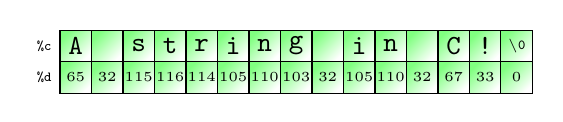
\begin{tikzpicture}[]
\foreach \x in {0.0, 0.4, ..., 5.6}
   \shadedraw [top color=green!50,shading angle=45] (\x,0) rectangle +(0.4,0.4);
\foreach \x in {0.0, 0.4, ..., 5.6}
   \shadedraw [top color=green!50,shading angle=45] (\x,0.4) rectangle +(0.4,0.4); \node at (0.2, 0.2) {\tiny65};
\node at (0.6, 0.2) {\tiny32};
\node at (1.0, 0.2) {\tiny115};
\node at (1.4, 0.2) {\tiny116};
\node at (1.8, 0.2) {\tiny114};
\node at (2.2, 0.2) {\tiny105};
\node at (2.6, 0.2) {\tiny110};
\node at (3.0, 0.2) {\tiny103};
\node at (3.4, 0.2) {\tiny32};
\node at (3.8, 0.2) {\tiny105};
\node at (4.2, 0.2) {\tiny110};
\node at (4.6, 0.2) {\tiny32};
\node at (5.0, 0.2) {\tiny67};
\node at (5.4, 0.2) {\tiny33};
\node at (5.8, 0.2) {\tiny0};

\node at (0.2, 0.6) {\tt A};
\node at (1.0, 0.6) {\tt s};
\node at (1.4, 0.6) {\tt t};
\node at (1.8, 0.6) {\tt r};
\node at (2.2, 0.6) {\tt i};
\node at (2.6, 0.6) {\tt n};
\node at (3.0, 0.6) {\tt g};
\node at (3.8, 0.6) {\tt i};
\node at (4.2, 0.6) {\tt n};
\node at (5.0, 0.6) {\tt C};
\node at (5.4, 0.6) {\tt !};
\node at (5.8, 0.6) {\tiny\tt $\backslash$0};

\node at (-0.2, 0.2) {\tiny\tt\%d};
\node at (-0.2, 0.6) {\tiny\tt\%c};
\end{tikzpicture}
\end{center}
\begin{itemize}
\item All strings in C are terminated by 0 (or {\tt \kt{'$\backslash$0'}}).
\item {\tt \kw{char}} values of 0-127 correspond to \emph{ASCII} codes, their use should be relatively consistent between different compilers.
\item All other values correspond to \emph{extended ASCII} codes, the representations of which vary considerably between compilers.
\end{itemize}
\end{frame}

\begin{frame}
\frametitle{Some useful String Functions}
\begin{block}{\tt strlen(s)}
Returns the number of characters pointed to by {\tt s}, the trailing {\tt NULL} ({\tt \kt{'$\backslash$0'}}) is excluded!
\end{block}
\begin{block}{\tt strncpy(dest, source, length)}
Copies a maximum of {\tt length} characters from {\tt source} to {\tt dest}.
\end{block}
\begin{block}{\tt int strncmp(s1, s2, length)}
Compares a maximum of {\tt length} characters of {\tt s1} and {\tt s2}. Note that {\tt strncmp} returns 0 (usually false) for equality!
\end{block}
\end{frame}

\begin{frame}[fragile]
\frametitle{A String Demo}
\vspace{-0.2in}
\begin{semiverbatim}
\tiny
\kr\kl\kw{\#include} \kt{<stdio.h>}
\kl\kw{\#include} \kt{<string.h>}
\kl\kw{\#include} \kt{<stdlib.h>}
\kl\kw{\#include} \kt{<ctype.h>}
\kl
\kl\kw{int} main()
\kl\{
\kl   \kw{unsigned int} loop;
\kl   \kw{char} * string = \kt{"A string in C!"}, * copy;
\kl   printf(\kt{"strlen(string) = \%d\\n"}, strlen(string));
\kl   copy = (char *) calloc(strlen(string)+1, 1);
\kl   \kw{if} (!copy)
\kl   \{
\kl      fprintf(stderr, \kt{"Couldn't allocate buffer!\\n"});
\kl      \kw{return} -1;
\kl   \}
\kl   
\kl   strncpy(copy, string, strlen(string));
\kl   printf(\kt{"strncmp(string, copy) = \%d\\n"},
\kl         strncmp(string, copy, strlen(string)));
\kl         
\kl   \kw{for} (loop = 0; loop < strlen(copy); loop++)
\kl      copy[loop] = toupper(copy[loop]);
\kl      
\kl   printf(\kt{"modified copy = \\"\%s\\"\\n"}, copy);
\kl   printf(\kt{"strncmp(string, copy) = \%d\\n"},
\kl         strncmp(string, copy, strlen(string)));
\kl         
\kl   free(copy);
\kl   \kw{return} 0;
\kl\}
\end{semiverbatim}
\end{frame}

\begin{frame}[fragile]
\frametitle{Results from String Demo}
The program on the previous slide gives the following output:
\begin{semiverbatim}
strlen(string) = 14
strncmp(string, copy) = 0
modified copy = "A STRING IN C!"
strncmp(string, copy) = 32
\end{semiverbatim}
\begin{itemize}
\item Note that {\tt strncmp} returns {\tt 0} for \emph{equality} and non-zero otherwise.
\item Case insensitive string comparisons can be made using: {\tt strnicmp}.
\end{itemize}
\end{frame}



\section{Streams}
\subsection{Standard Streams}
\begin{frame}
\frametitle{Input and Output in C - Streams}
\begin{itemize}
\item All I/O in C is accomplished via file \emph{streams}.
\item This stems from C's UNIX roots (every device is a file).
\item We have already seen {\tt printf}, formatted output to console.
\item C90 defines three streams which are initialised by default when a program starts.
\begin{center}
\rowcolors[]{1}{blue!20}{blue!10}
\begin{tabular}{l l}
{\tt stdin}&Input from the keyboard. (read only)\\
{\tt stdout}&Text console. (write only)\\
{\tt stderr}&Another text console. (write only)
\end{tabular}
\end{center}
\end{itemize}
\end{frame}

\begin{frame}
\frametitle{Why have {\tt stderr}?}
\begin{exampleblock}{Stream Redirection}
\begin{itemize}
\item UNIX (and now most other operating systems) allow for a C program's streams to be \emph{redirected} at the command line.
\item This is completely transparent to the C program (it just reads and writes data oblivious to the source).
\item One can redirect {\tt stdout} using ({\tt >}) as follows:
\begin{center}
\tt myprogram > output.txt
\end{center}
\item {\tt stderr} can be redirected using ({\tt 2>}):
\begin{center}
\tt myprogram 2> errorlog.txt
\end{center}
\item {\tt stdin} can be redirected using ({\tt <}):
\begin{center}
\tt myprogram < input.txt
\end{center}
\end{itemize}
\end{exampleblock}
Having a separate \emph{error stream}, allows for important messages to be filtered from data output.
\end{frame}


\begin{frame}[fragile]
\frametitle{{\tt printf} and {\tt scanf} - formatted output and input}
These are automatically connected to {\tt stdout} and {\tt stderr} respectively. The more generalised functions are {\tt fprintf} and {\tt fscanf}. As an example:
\begin{semiverbatim}
fprintf(stdout, \kt{"Text to stdout...\\n"});
fprintf(stderr, \kt{"Text to stderr...\\n"});
\end{semiverbatim}
We can also read text from a stream:
\begin{semiverbatim}
fscanf(stdin, \kt{"%lf"}, \&ptrDouble);
\end{semiverbatim}
\begin{itemize}
\item Additional streams can be opened using {\tt fopen}.
\end{itemize}
\end{frame}

\subsection{Opening Files}
\begin{frame}
\frametitle{{\tt fopen} - open a file stream}
\begin{semiverbatim}
\small
FILE * stream = fopen(\kw{char} * filename, \kw{char} * mode);
\end{semiverbatim}

Working backwards, {\tt mode} is a string telling C how to open the file:
{\footnotesize
\begin{center}
\rowcolors[]{1}{blue!20}{blue!10}
\begin{tabular}{l p{250pt}}
\tt mode& meaning\\
\tt "r"& Open {\tt filename} for reading. The file must exist or {\tt NULL} is returned.\\
\tt "w"& Open {\tt filename} for writing, starting from the beginning of the file. The file will be created if it doesn't already exist. Any old data will be overwritten.\\
\tt "a"& Open {\tt filename} for writing, starting from the end of the file. File will be \emph{appended} if it doesn't exist and created otherwise.\\
\tt "r+"& Open {\tt filename} for reading and writing, starting from the beginning. If the file doesn't exist, {\tt NULL} is returned.\\
\tt "w+"& Open {\tt filename} for reading and writing, starting from the beginning. If the file doesn't exist it's created.\\
\tt "a+"& Open {\tt filename} for reading and writing (append if exists).
\end{tabular}
\end{center}}
\end{frame}

\begin{frame}[fragile]
\frametitle{{\tt fopen} - II}
\begin{semiverbatim}
\small
FILE * stream = fopen(\kw{char} * filename, \kw{char} * mode);
\end{semiverbatim}
\begin{block}{\tt filename}
Must be a legal operating system file name. A safe option would be something similar to:
\vspace{-0.1in}
\begin{center}
\tt \kt{"results.txt"}
\end{center}
\end{block}

\begin{alertblock}{Absolute Filenames}
We can specify a full directory path to a filename:
\vspace{-0.2in}
\begin{semiverbatim}
\footnotesize
data = fopen(\kt{"C:\\\\TEMP\\\\mydata.dat"}, \kt{"w"}); \kc{/* Windows */}
data = fopen(\kt{"/tmp/mydata.dat"}, \kt{"w"});      \kc{/* UNIX */}
\end{semiverbatim}
\end{alertblock}

\begin{exampleblock}{Relative Filenames}
It is much safer to omit the full path:
\vspace{-0.2in}
\begin{semiverbatim}
\footnotesize
data = fopen(\kt{"mydata.dat"}, \kt{"w"}); \kc{/* works on most os' */}
\end{semiverbatim}
\end{exampleblock}
\end{frame}

\begin{frame}[fragile]
\frametitle{{\tt fopen} - III}
\begin{semiverbatim}
\small
FILE * stream = fopen(\kw{char} * filename, \kw{char} * mode);
\end{semiverbatim}
\vspace{-0.1in}
\begin{itemize}
\item Here {\tt stream} is a pointer to a {\tt FILE} data type.
\item {\tt stdin}, {\tt stdout} and {\tt stderr} are also pointers (which are opened automatically for us).
\item Sometimes it is not possible to open a file (it may not exist, or belong to another user etc...), in this case a special pointer value {\tt NULL} (which is equal to zero) is returned.
\end{itemize}

\begin{block}{{\tt NULL} pointers}
A {\tt NULL} pointer is a special value, usually signalling failure. This can be checked for:
\vspace{-0.2in}
\begin{semiverbatim}
\footnotesize
stream = fopen(\kt{"illegal/\\\\filename.txt"}, \kt{"w"});
if (!stream)
\{
   fprintf(stderr, \kt{"Unable to open file\\n"});
   ...
\end{semiverbatim}
\end{block}
\end{frame}

\begin{frame}
\frametitle{{\tt fclose} - Closing a file stream}
\begin{itemize}
\item Any file streams {\tt fopen}'ed should be closed using:
\begin{center}
\tt fclose(stream);
\end{center}
\begin{itemize}
\item File read/writes may go to an internal buffer before they go to the disk (to speed things up).
\item An explicit file close ensures that any pending data is written to disk.
\end{itemize}
\item For the lazy there is:
\begin{center}
\tt fcloseall();
\end{center}
\item Do \emph{NOT} call {\tt fclose} on any of the following:
\begin{center}
{\tt stdin, stdout} \& \tt stderr
\end{center}
\end{itemize}
\end{frame}

\begin{frame}
\frametitle{Moving around a file - {\tt rewind}, {\tt ftell} and {\tt fseek}}
\begin{block}{\tt rewind(stream);}
Start the next read/write from the beginning of the file.
\end{block}

\begin{block}{\tt fpos = ftell(stream);}
Get an \kw{\tt int} telling us how far we are in the file (from the beginning).
\end{block}

\begin{block}{\tt fseek(stream, fpos, SEEK\_SET);}
Move {\tt fpos} bytes into the file (counted from the beginning).
\end{block}

\begin{block}{\tt fseek(stream, fpos, SEEK\_CUR);}
Move {\tt fpos} bytes forward into file (from current position).
\end{block}

\begin{block}{\tt fseek(stream, fpos, SEEK\_END);}
Move {\tt fpos} bytes from the end of the file.
\end{block}
\end{frame}

\subsection{File Types}
\begin{frame}
\frametitle{File Types}
Files in C can contain data in two formats:
\begin{enumerate}
\item As text, where each byte is interpreted as an ASCII character mapping.
\item Or as raw \emph{binary} data, the meaning of which is left to the program to determine.
\end{enumerate}

These files are referred to as text files and binary files respectively. All the I/O covered so far applies to text files.

\begin{block}{}
\begin{center}
Each format has it's advantages and disadvantages.
\end{center}
\end{block}
\end{frame}

\begin{frame}
\frametitle{Text versus Binary Files}
\begin{block}{Text Files}
\begin{itemize}
{\setbeamercolor{local structure}{parent=example text}
\item \textcolor{green}{Pro} - Can be read by almost any program on almost any computer. (And by humans!).
}
{\setbeamercolor{local structure}{parent=alerted text}
\item \textcolor{red}{Con} - Inefficient - Numbers can take up as much as twice the space as necessary.}
\end{itemize}
\end{block}

\begin{block}{Binary Files}
\begin{itemize}
{\setbeamercolor{local structure}{parent=example text}
\item \textcolor{green}{Pro} - Accurate and efficient.
}
{\setbeamercolor{local structure}{parent=alerted text}
\item \textcolor{red}{Con} - Incompatible - Binary data can be very difficult to read by other programs, and incredibly difficult between processor architectures.}
\end{itemize}
\end{block}
\end{frame}

\subsection{Binary Files}
\begin{frame}[fragile]
\frametitle{Variable sizes}
\begin{itemize}
\item Different data types take up different amounts of memory.
\item Example \kw{\tt float} is smaller than \kw{\tt double}.
\item The \kw{\tt sizeof} keyword gives a type's size (in bytes).
\end{itemize}

{
\small
\begin{semiverbatim}
\kw{\#include} \kt{<stdio.h>}

\kw{int} main()
\{
   printf(\kt{"sizeof(float) = \%d\\n"}, \kw{sizeof}(\kw{float}));
   printf(\kt{"sizeof(double) = \%d\\n"}, \kw{sizeof}(\kw{double}));
   printf(\kt{"sizeof(int) = \%d\\n"}, \kw{sizeof}(\kw{int}));
   printf(\kt{"sizeof(short) = \%d\\n"}, \kw{sizeof}(\kw{short}));
   \kw{return} 0;
\}
\end{semiverbatim}
}
\end{frame}

\begin{frame}[fragile]
\frametitle{Handling Binary Files}
Binary files are opened using {\tt fopen}, we need to add {\tt "b"} to the file mode though:
\begin{semiverbatim}
stream = fopen(\kt{"data.dat"}, \kt{"rb"});
\end{semiverbatim}
Data is read from and written to a binary file using {\tt fread} and {\tt fwrite}. For example:
\begin{semiverbatim}
\kw{double} values[10] = \{0.0\};
\kc{/* we have "stream" an open binary file */}
read = fread(values, \kw{sizeof}(\kw{double}), 10, stream);
\kw{if} (read != 10)
\{ \emph{read failed} \}
\end{semiverbatim}
\begin{block}{}
\begin{center}
Please see \kt{\tt <stdio.h>} for more details.
\end{center}
\end{block}
\end{frame}

\subsection{Temporary Files}
\begin{frame}[fragile]
\frametitle{Permanent versus Temporary Files}
\begin{itemize}
\item Sometimes we may not wish for a file to be permanent.
\item Temporary files provide a means for storing intermediate computations.
\item We open a temporary file using the {\tt tmpfile()} function.
\end{itemize}
\begin{block}{Example}
\begin{semiverbatim}
stream = tmpfile();
\kw{if} (!stream)
\{
\kc{/* handle failure */}
\}
\kc{/* fread, fwrite, fprintf, fscanf */}
fclose(stream);
\end{semiverbatim}
\end{block}
\end{frame}


\section{Allocation Memory}
\subsection{Borrowing From the Heap}
\begin{frame}
\frametitle{Dynamic Allocation}
\begin{block}{The heap}
\begin{itemize}
\item C has set aside a special block of memory known as the \emph{heap}.
\item Memory can be requested from the heap.
\item If memory is available, it is provided, otherwise a request is made to the operating system.
\item The implementation details of the heap are ``undefined''.
\end{itemize}
\end{block}
\begin{block}{\tt sizeof}
\begin{itemize}
\item We need to know how much memory to request.
\item The \kw{\tt sizeof} keyword returns the size (in bytes), of a variable or data type.
\end{itemize}
\end{block}
\end{frame}

\begin{frame}[fragile]
\frametitle{How to Borrow Memory}
We use the {\tt malloc} function (defined in \kt{\tt <stdlib.h>}) to request memory and {\tt free} to return it to the heap.
\vspace{-0.1in}
\begin{semiverbatim}
\scriptsize
\kr\kl\kw{\#include} \kt{<stdio.h>}
\kl\kw{\#include} \kt{<stdlib.h>}
\kl\kw{\#define} NCOUNT 10
\kl\kw{int} main()
\kl\{
\kl   \kw{int} * numbers, loop;
\kl   numbers = (\kw{int} *) malloc(\kw{sizeof}(\kw{int})*NCOUNT);
\kl   \kw{if} (!numbers)
\kl   \{
\kl      fprintf(stderr, \kt{"Unable to allocate memory\\n"});
\kl      return -1;
\kl   \}
\kl   \kw{for} (loop = 0; loop < NCOUNT; loop++)
\kl      numbers[loop] = loop;
\kl
\kl   \kw{for} (loop = 0; loop < NCOUNT; loop++)
\kl      printf(\kt{"numbers[\%d] = \%d\\n"}, loop, numbers[loop]);
\kl
\kl   \kw{free}(numbers);
\kl   \kw{return} 0;
\kl\}
\end{semiverbatim}
\end{frame}

\begin{frame}[fragile]
\frametitle{How to Borrow Memory - Details}
\begin{semiverbatim}
      \kw{void} * malloc(size_t Size);
      \kw{void} free(\kw{void} * Memory);
\end{semiverbatim}
\begin{block}{What is {\tt void *}?}
\begin{itemize}
\item {\tt \kw{void} *} is a pointer to an unknown data type, it consists only of an address.
\item We can explicitly cast from {\tt \kw{void} *} to any other pointer type.
\item Any pointer type can be implicitly casted to a {\tt \kw{void} *}.
\item A value of {\tt NULL} usually means that a function encountered an error.
\end{itemize}
\end{block}

\begin{block}{What is {\tt size\_t}?}
{\tt size\_t} is defined to be an unsigned integer type large enough to hold numbers returned by {\tt \kw{sizeof}}.
\end{block}
\end{frame}

\begin{frame}
\frametitle{How to Borrow Memory - More Details}
Two more popular memory management functions are:
\begin{center}
\rowcolors[]{1}{blue!20}{blue!10}
\begin{tabular}{l l}
\tt realloc&Modifies the size of a memory block.\\
\tt calloc&Allocates memory, and sets every byte to 0.\\
\end{tabular}
\end{center}
\begin{alertblock}{Some common heap problems}
\begin{itemize}
\item Allocating memory is slow and should be done as few times as possible.
\item Memory allocation can fail, every {\tt malloc}/{\tt calloc} should be checked (or at the very least {\tt assert}ed).
\item Every {\tt malloc}/{\tt calloc} should have a corresponding {\tt free}, memory is \emph{leaked} if it's not {\tt free}d after use.
\end{itemize}
\end{alertblock}
\end{frame}

\begin{frame}[fragile]
\frametitle{1-D Example: Fibonacci (again!)}
\begin{semiverbatim}
\tiny
\kr\kl\kw{\#include} \kt{<stdlib.h>}
\kl\kw{\#include} \kt{<stdio.h>}
\kl
\kl\kw{int} main()
\kl\{
\kl   \kw{double} * fibs;
\kl   \kw{unsigned int} nfibs=0, loop;
\kl   \kw{while} (nfibs < 2)
\kl   \{
\kl      printf(\kt{"How many Fibonacci numbers are needed (>1)?\\n"});
\kl      scanf(\kt{"\%u"}, \&nfibs);
\kl   \}
\kl   
\kl   fibs = (\kw{double} *) malloc(\kw{sizeof}(\kw{double})*nfibs);
\kl   \kw{if} (!fibs) \kc{/* malloc failed? */}
\kl   \{
\kl      fprintf(stderr, \kt{"Unable to allocate memory!\\n"});
\kl      \kw{return} -1;
\kl   \}       
\kl   
\kl   fibs[0] = 1.0; fibs[1] = 1.0;
\kl   \kw{for} (loop = 2; loop < nfibs; loop++)
\kl      fibs[loop] = fibs[loop-1]+fibs[loop-2];
\kl      
\kl   \kw{for} (loop = 0; loop < nfibs; loop++)
\kl      printf(\kt{"fib[\%u] = \%lg\\n"}, loop, fibs[loop]);
\kl      
\kl   free(fibs);
\kl   \kw{return} 0;
\kl\}
\end{semiverbatim}
\end{frame}

\begin{frame}
\frametitle{Pointers to Pointers: {\tt **ptr}}
\begin{itemize}
\item Pointers in C are very flexible, to the extent that we can form pointers to pointers!
\item This is known more formally as the ``level of indirection''.
\item Tensors of arbitrary rank (Fortran 95 is limited to 7) can be formed easily in C.
\item The most useful example in C being matrices.
\end{itemize}
\begin{block}{Matrices in C}
Matrices in C are commonly represented by the {\tt \kw{double} **} type. This means ``a pointer to a pointer to a {\tt \kw{double}}''.
\end{block}
\end{frame}


\section{Matrices}
\subsection{Pointers III}
\begin{frame}[fragile]
\frametitle{Pointers and Arrays}
We saw the connection between arrays and pointers in the last lecture. Given the array:
\begin{center}
\tt \kw{double} ar [4] = \{1.0, 2.0, 3.0, 4.0\};
\end{center}
The elements of this array can be accessed as follows:
\begin{semiverbatim}
      *(ar) == ar[0] == 1.0
    *(ar+1) == ar[1] == 2.0
    *(ar+2) == ar[2] == 3.0
\end{semiverbatim}
Pointer referencing is also supported:
\begin{semiverbatim}
        ar == \&ar[0]
    (ar+1) == \&ar[1]
    (ar+2) == \&ar[2]
\end{semiverbatim}
\end{frame}

\begin{frame}
\frametitle{Allowed Pointer Operations}
\begin{tabular}{l l}
Declaration:&{\tt \kw{double} * pA, * pB;}\\
Assignment:&{\tt pA = \&var;}\\
Increment:&{\tt pA = pA + 1;}\\
Decrement:&{\tt pA = pA - 1;}\\
Difference:&{\tt gap = pA - pB;}\\
Comparison:&{\tt \kw{if}(pA == pB)}\\
De-referencing:&{\tt *pA = val;}
\end{tabular}
\end{frame}

\subsection{Fixed Sized Matrices}
\begin{frame}[fragile]
\frametitle{Fixed Size Two-Dimensional Arrays}
We can declare arrays of dimension higher than one, as follows:
\begin{semiverbatim}
\kw{double} a[2][3] = \{\{1.0, 2.0, 3.0\},
                  \{2.0, 3.0, 4.0\}\};
\end{semiverbatim}
Where the elements of {\tt a} are denoted as expected:
\begin{center}
\begin{tabular}{|c|c|c|}
\hline
\tt a[0][0]&\tt a[0][1]&\tt a[0][2]\\
\hline
\tt a[1][0]&\tt a[1][1]&\tt a[1][2]\\
\hline
\end{tabular}
\end{center}
To access the top left element:
\begin{semiverbatim}
myVal = a[0][0]; \kc{/* equal to 1.0 */}
\end{semiverbatim}
\end{frame}

\begin{frame}[fragile]
\frametitle{Fixed Size Two-Dimensional Arrays II}
\vspace{-0.2in}
\begin{semiverbatim}
\footnotesize
\kr\kl\kw{\#include} \kt{<stdio.h>}
\kl\kw{\#define} COLS 3
\kl
\kl\kw{void} printArray(\kw{int} matrix[][COLS], int rows)
\kl\{
\kl   \kw{int} i, j;
\kl   \kw{for} (i = 0; i < rows; i++)
\kl   \{
\kl      \kw{for} (j = 0; j < COLS; j++)
\kl         printf(\kt{"\%d "}, matrix[i][j]);    
\kl      printf(\kt{"\\n"});
\kl   \}
\kl\}
\kl
\kl\kw{int} main()
\kl\{
\kl   \kw{int} matrix[2][COLS] = \{\{1, 2, 3\},\{4, 5, 6\}\};
\kl   printArray(matrix, 2);
\kl   \kw{return} 0;
\kl\}
\end{semiverbatim}
\end{frame}

\begin{frame}
\frametitle{Fixed Size Two-Dimensional Arrays III}
We have seen an example of a two dimensional array:
\begin{center}
%\rowcolors[]{1}{blue!20}{blue!10}
\begin{tabular}{|c|c|c|}
\hline
\tt a[0][0]&\tt a[0][1]&\tt a[0][2]\\
\hline
\tt a[1][0]&\tt a[1][1]&\tt a[1][2]\\
\hline
\end{tabular}
\end{center}
\begin{itemize}
\item In memory it is arranged as follows:
\resizebox{0.9\textwidth}{!}{
\begin{tabular}{|c|c|c|c|c|c|}
\hline
\tt a[0][0]&\tt a[0][1]&\tt a[0][2]&
\tt a[1][0]&\tt a[1][1]&\tt a[1][2]\\
\hline
\end{tabular}}
(i.e. as a one dimensional array).
\item Fixed size arrays are very inflexible as they require the dimensions to be ``hard coded''.
\item They are allocated from the stack thus large arrays may cause problems.
\item \emph{Dynamically allocated} arrays overcome these restrictions.
\end{itemize}
\end{frame}

\subsection{Dynamically Allocating Matrices}
\begin{frame}[fragile]
\frametitle{Constructing Matrices with Pointers}
\vspace{-0.2in}
\begin{semiverbatim}
\footnotesize
\kr\kl\kw{double} ** makeMatrix(\kw{unsigned int} rows, \kw{unsigned int} cols)
\kl\{
\kl   \kw{unsigned int} i;
\kl   \kw{double} ** matrix;
\kl        
\kl   matrix = (\kw{double} **) malloc(rows * \kw{sizeof}(\kw{double} *));
\kl   \kw{if} (!matrix) \kw{return} NULL; \kc{/* failed */}
\kl
\kl   \kw{for} (i = 0; i < rows; i++)
\kl   \{
\kl      matrix[i] = (\kw{double} *) malloc(cols*\kw{sizeof}(\kw{double}));
\kl      \kw{if} (!matrix[i])
\kl         \kw{return} NULL; \kc{/* lazy, we should really free} 
\kl                         \kc{all the memory allocated above */}
\kl   \}
\kl
\kl   \kw{return} matrix;
\kl\}
\end{semiverbatim}
\end{frame}

\begin{frame}[fragile]
\frametitle{Accessing Matrix Elements}
\begin{block}{Usage pattern for {\tt makeMatrix}}
\begin{semiverbatim}
\kw{double} ** matrix = makeMatrix(rows, cols);
\kw{for} (i=0; i < rows; i++)
   \kw{for} (j=0; j < cols; j++)
      matrix[i][j] = 0.0;
\emph{free the matrix}      
\end{semiverbatim}
\end{block}
\begin{itemize}
\item Accessing the dynamically allocated array looks identical to the fixed size ones, but ``under the hood'' things are a little different:
\begin{alertblock}{}
\begin{center}
\tt matrix[row][col] = *(*(matrix + row) + col)
\end{center}
\end{alertblock}
\item The {\tt makeMatrix} code on the previous slide contained a lot of {\tt malloc} statements, is there a better way to allocate a matrix? (yes!)
\end{itemize}
\end{frame}

\begin{frame}[fragile]
\frametitle{A Better Way of Allocating Matrices}
\begin{semiverbatim}
\scriptsize
\kr\kl\kw{double} ** allocMatrix(\kw{unsigned int} rows, \kw{unsigned int} cols)
\kl\{
\kl   \kw{double} ** matrix;
\kl   \kw{unsigned int} i;
\kl
\kl   matrix = (\kw{double} **) malloc (rows*sizeof(\kw{double} *));
\kl   \kw{if} (!matrix) \kw{return} NULL; \kc{/* failed */}
\kl
\kl   matrix[0] = (\kw{double} *) malloc (rows*cols*\kw{sizeof}(\kw{double}));
\kl   \kw{if} (!matrix[0])
\kl   \{
\kl      free(matrix); \kc{/* we don't need matrix any more */}
\kl      \kw{return} NULL;  \kc{/* failed */}
\kl   \}
\kl
\kl   \kw{for} (i = 1; i < rows; i++)
\kl      matrix[i] = matrix[i-1] + cols;
\kl
\kl   \kw{return} matrix;
\kl\}
\end{semiverbatim}
\end{frame}

\begin{frame}[fragile]
\frametitle{Why is {\tt allocMatrix} Better?}
\begin{itemize}
\item {\tt allocMatrix} only uses 2 {\tt malloc}s whilst, {\tt makeMatrix} uses {\tt cols + 1}.
\item Meaning there are fewer points of failure (we only check two pointers for {\tt NULL}),
\item It is much easier to free a matrix allocated with the {\tt allocMatrix} function, all we need to do is:
\begin{semiverbatim}
\kw{void} freeMatrix(\kw{double} ** matrix)
\{
   free(matrix[0]);
   free(matrix);
\}
\end{semiverbatim}
\end{itemize}
\end{frame}

\subsection{Working with Matrices}
\begin{frame}
\frametitle{Case Study: Matrix Addition}
Let's define some utility functions to:
\begin{enumerate}
\item Allocate memory for the matrix ({\tt allocMatrix}) - {\bf done},
\item Free a matrix ({\tt freeMatrix}) - {\bf done},
\item Print a matrix ({\tt printMatrix}),
\item Create a random matrix ({\tt randomMatrix}),
\item Add matrices together ({\tt addMatrices})
\end{enumerate}
We drive all these functions using a {\tt main} function.
\end{frame}

\begin{frame}[fragile]
\frametitle{{\tt printMatrix} and {\tt randomMatrix}}
\begin{semiverbatim}
\scriptsize
\kr\kl\kw{void} printMatrix(\kw{double} ** matrix, \kw{unsigned int} rows,
\kl                                   \kw{unsigned int} cols)
\kl\{
\kl   \kw{unsigned int} i, j;
\kl
\kl   \kw{for} (i = 0; i < rows; i++)
\kl   \{
\kl      \kw{for} (j = 0; j < cols; j++)
\kl         printf(\kt{"\%8.5lf "}, matrix[i][j]);
\kl      printf(\kt{"\\n"});
\kl   \}
\kl\}
\end{semiverbatim}

\begin{semiverbatim}
\scriptsize
\kr\kl\kw{void} randomMatrix(\kw{double} ** matrix, \kw{unsigned int} rows,
\kl                                    \kw{unsigned int} cols)
\kl\{
\kl   \kw{unsigned int} i, j;
\kl   \kw{for} (i = 0; i < rows; i++)
\kl      \kw{for} (j = 0; j < cols; j++)
\kl         matrix[i][j] = (\kw{double})rand()/RAND_MAX;
\kl\}
\end{semiverbatim}
\end{frame}

\begin{frame}[fragile]
\frametitle{{\tt addMatrices}}
\begin{semiverbatim}
\scriptsize
\kr\kl\kw{void} addMatrices(\kw{double} ** matrixA, \kw{double} ** matrixB,
\kl                 \kw{double} ** matrixR,
\kl                 \kw{unsigned int} rows, \kw{unsigned int} cols)
\kl\{
\kl   \kw{unsigned int} i, j;
\kl   \kw{for} (i = 0; i < rows; i++)
\kl      \kw{for} (j = 0; j < rows; j++)
\kl         matrixR[i][j] = matrixA[i][j]+matrixB[i][j];
\kl\}
\end{semiverbatim}
\end{frame}

\begin{frame}[fragile]
\frametitle{The {\tt main} function}
\begin{semiverbatim}
\tiny
\kr\kl\kw{int} main()
\kl\{
\kl   \kw{unsigned int} rows, cols;
\kl   \kw{double} ** matrixA, ** matrixB, **matrixC;
\kl   printf(\kt{"Enter rows cols: "});
\kl   scanf(\kt{"%u %u"}, &rows, &cols);
\kl
\kl   matrixA = allocMatrix(rows, cols);
\kl   matrixB = allocMatrix(rows, cols);
\kl   matrixC = allocMatrix(rows, cols);
\kl
\kl   \kw{if} (!matrixA || !matrixB || !matrixC)
\kl   \{   \kc{/* a little lazy, but it does the job */}
\kl      fprintf(stderr, \kt{"Unable to allocate matrices!\\n"});
\kl      \kw{return} -1;
\kl   \}
\kl
\kl   randomMatrix(matrixA, rows, cols); randomMatrix(matrixB, rows, cols);
\kl   addMatrices(matrixA, matrixB, matrixC, rows, cols);
\kl
\kl   printf(\kt{"\\n\\nmatrix A = \\n"});
\kl   printMatrix(matrixA, rows, cols);
\kl   printf(\kt{"\\n\\nmatrixB = \\n"});
\kl   printMatrix(matrixB, rows, cols);
\kl   printf(\kt{"\\n\\nmatrixA + matrixB = \\n"});
\kl   printMatrix(matrixC, rows, cols);
\kl
\kl   freeMatrix(matrixC); freeMatrix(matrixB); freeMatrix(matrixA);
\kl   \kw{return} 0;
\kl\}
\end{semiverbatim}
\end{frame}

\begin{frame}[fragile]
\frametitle{Results}
\vspace{-0.2in}
\begin{semiverbatim}
\scriptsize
Enter rows cols: 4 4


matrix A =
 0.00125  0.56359  0.19330  0.80874
 0.58501  0.47987  0.35029  0.89596
 0.82284  0.74660  0.17411  0.85894
 0.71050  0.51353  0.30399  0.01498


matrixB =
 0.09140  0.36445  0.14731  0.16590
 0.98853  0.44569  0.11908  0.00467
 0.00891  0.37788  0.53166  0.57118
 0.60176  0.60717  0.16623  0.66305


matrixA + matrixB =
 0.09265  0.92804  0.34062  0.97464
 1.57353  0.92557  0.46937  0.90063
 0.83175  1.12449  0.70577  1.43013
 1.31227  1.12070  0.47023  0.67803
\end{semiverbatim}
\end{frame}

\begin{frame}
\frametitle{Matrices - Details}
\framesubtitle{For matrices allocated in the previous lecture}
\begin{tabular}{l l}
\tt matrix & points to a matrix\\
\tt matrix[0]& points to the first row of the matrix\\
\tt matrix[0][0]&The top left element of the matrix
\end{tabular}\\
\vspace{0.2in}
Which have the following types:\\
\begin{tabular}{l l}
\tt matrix& \tt \kw{double} **\\
\tt matrix[0]&\tt \kw{double} *\\
\tt matrix[0][0]& \tt \kw{double}
\end{tabular}
\end{frame}

\subsection{Higher Dimension Arrays}
\begin{frame}[fragile]
\frametitle{Higher Dimensional Arrays}
\begin{semiverbatim}
\tiny
\kr\kl\kw{double} *** alloc3Tensor(\kw{unsigned int} dim)
\kl\{
\kl   \kw{unsigned int} i, j;
\kl   \kw{double} *** tensor;
\kl   tensor = (\kw{double} ***) malloc(dim*\kw{sizeof}(\kw{double} **));
\kl   \kw{if} (!tensor) \kw{return} NULL;
\kl   tensor[0] = (\kw{double} **) malloc(dim*dim*\kw{sizeof}(\kw{double} *));
\kl   \kw{if} (!tensor[0])
\kl   \{
\kl      free(tensor);
\kl      \kw{return} NULL;
\kl   \}
\kl   tensor[0][0] = (\kw{double} *) malloc(dim*dim*dim*\kw{sizeof}(\kw{double}));
\kl   \kw{if} (!tensor[0][0])
\kl   \{
\kl      free(tensor[0]); free(tensor);
\kl      \kw{return} NULL;
\kl   \}
\kl   \kw{for} (i = 1; i < dim; i++)
\kl      tensor[0][i] = tensor[0][i-1]+dim;
\kl   \kw{for} (i = 1; i < dim; i++)
\kl   \{
\kl      tensor[i] = tensor[i-1] + dim;
\kl      tensor[i][0] = tensor[i-1][0] + dim * dim;
\kl      \kw{for} (j = 1; j < dim; j++)
\kl         tensor[i][j] = tensor[i][j-1] + dim;
\kl   \}
\kl   \kw{return} tensor;
\kl\}
\end{semiverbatim}
\end{frame}

\begin{frame}[fragile]
\frametitle{More Multi-Index}
\begin{itemize}
\item The 3D array behaves as expected:\\
\begin{center}
\tt tensor[i][j][k] = 0.5;
\end{center}
\item The array can be freed with:
\begin{semiverbatim}
\kw{void} free3Tensor(\kw{double} *** tensor)
\{
   free(tensor[0][0]);
   free(tensor[0]);
   free(tensor);
\}
\end{semiverbatim}
\end{itemize}
\end{frame}

\subsection{Non-'Square' Arrays}
\begin{frame}
\frametitle{More Elaborate Data Structures}
\begin{itemize}
\item In C we are able to manipulate data directly, this has allowed us to partition a contiguous array of memory into matrix rows.
\item We needn't restrict ourselves to structures where the number of elements per row is constant, one example is Pascal's triangle:\\
\begin{center}
\tt1\\\tt1  2  1\\\tt1  3  3  1\\\tt1  4  6  4  1\\$\vdots$
\end{center}
\end{itemize}
\end{frame}

\begin{frame}[fragile]
\begin{semiverbatim}
\scriptsize
\kr\kl\kw{int} main()
\kl\{
\kl   \kw{unsigned int} size = 10, r, c;
\kl   \kw{int} ** pasc;
\kl   pasc = (\kw{int} **) malloc(size*sizeof(int));
\kl   pasc[0] = (\kw{int} *) malloc(size*(size+1)*sizeof(int)/2);
\kl   \kc{/* check the mallocs */}
\kl   \kw{for} (r=1; r < size; r++) pasc[r] = pasc[r-1]+r;
\kl   pasc[0][0] = 1;
\kl   \kw{for} (r = 1; r < size; r++)
\kl   \{
\kl      \kw{for} (c = 1; c < r; c++)
\kl         pasc[r][c] = pasc[r-1][c-1]+pasc[r-1][c];
\kl      pasc[r][0] = 1; pasc[r][r] = 1;
\kl   \}
\kl   \kw{for} (r=0; r < size; r++)
\kl   \{
\kl      \kw{for} (c = 0; c < r+1; c++)
\kl         printf(\kt{"\%3d "}, pasc[r][c]);
\kl      printf(\kt{"\\n"});
\kl   \}
\kl   free(pasc[0]);
\kl   free(pasc);
\kl   \kw{return} 0;
\kl\}
\end{semiverbatim}
\end{frame}

\begin{frame}[fragile]
\frametitle{Pascal's Triangle}
\begin{itemize}
\item The program outputs:
\vspace{-0.2in}
\begin{semiverbatim}
\small
  1
  1   1
  1   2   1
  1   3   3   1
  1   4   6   4   1
  1   5  10  10   5   1
  1   6  15  20  15   6   1
  1   7  21  35  35  21   7   1
  1   8  28  56  70  56  28   8   1
  1   9  36  84 126 126  84  36   9   1
\end{semiverbatim}
\item Whilst in memory, the data structure looks like:
\begin{tabular}{|c|c|c|c|c|c|c|c|c|c|c|}
\hline
\tt1&\tt1&\tt1&\tt1&\tt2&\tt1&\tt1&\tt3&\tt3&\tt1&$\cdots$\\
\hline
\end{tabular}
\end{itemize}
\end{frame}


\section{Scructs}
\subsection{Custom Data Types}
\begin{frame}[fragile]
\frametitle{Custom Data Types}
Recall, when dealing with files we used:
\begin{semiverbatim}
FILE * file;
file = fopen (\kt{"myfile.txt"}, \kt{"r"});
\end{semiverbatim}
{\tt FILE} is in fact a custom data type, with its own size:
\begin{semiverbatim}
\kw{\#include} \kt{<stdio.h>}

\kw{int} main()
\{
   printf(\kt{"sizeof(FILE) = \%d\\n"}, \kw{sizeof}(FILE));
   \kw{return} 0;
\}
\end{semiverbatim}
\end{frame}

\begin{frame}[fragile]
\frametitle{Except from MS - \kt{\tt <stdio.h>}}
(From Visual Studio 2008)
\begin{semiverbatim}
\kw{struct} _iobuf \{
   \kw{char} *_ptr;
   \kw{int}   _cnt;
   \kw{char} *_base;
   \kw{int}   _flag;
   \kw{int}   _file;
   \kw{int}   _charbuf;
   \kw{int}   _bufsiz;
   \kw{char} *_tmpfname;
   \};
\kw{typedef struct} _iobuf FILE;
\end{semiverbatim}
\end{frame}

\subsection{Defining Our Structs}
\begin{frame}[fragile]
\frametitle{{\tt typedef} Structures : Custom Data Types}
\begin{itemize}
\item {\tt FILE} is a custom data type defined in \kt{\tt <stdio.h>}.
\item It is comprised of elements of different, known, types.
\item Each element of the {\tt FILE} \emph{structure} has its own name.
\end{itemize}

Let's consider a structure of our own, one of the simplest examples is a complex number:
\begin{columns}
\begin{column}{5cm}
\begin{semiverbatim}
\kw{typedef struct}
\{
   \kw{double} real;
   \kw{double} imag;
\} complex;
\end{semiverbatim}
\end{column}
\begin{column}{5cm}
\begin{alertblock}{C99}
C99 fully supports its own {\tt complex}
type.
\end{alertblock}
\end{column}
\end{columns}
\end{frame}

\begin{frame}[fragile]
\frametitle{{\tt typedef} Structures - II}
Definitions of structures take the following form:
\begin{semiverbatim}
   \kw{typedef struct}
   \{
      \emph{elementType} \emph{elementName};
      \emph{elementType} \emph{elementName};
      \vdots
   \} \emph{structureTypeName} ;
\end{semiverbatim}
\end{frame}

\subsection{Using Structures}
\begin{frame}
\frametitle{Handling Structures}
\begin{enumerate}
\item A structure may be an argument to a function.
\item A function may return a structure.
\item A pointer may point to a structure.
\item Structures are referenced as normal: {\tt \&name}.
\item Elements of a structure are references as: {\tt \&name.element}.
\item A pointer to a structure may be passed to a function.
\item If {\tt p} is a pointer to a structure, then {\tt p->member} allows us to access it's members.
\end{enumerate}
\end{frame}

\begin{frame}[fragile]
\frametitle{Example Function Applying to Structures}
\vspace{-0.2in}
\begin{semiverbatim}
\scriptsize
\kr\kl\kw{\#include} \kt{<stdio.h>}
\kl
\kl\kw{typedef struct}
\kl\{
\kl   \kw{double} real;
\kl   \kw{double} imag;
\kl\} complex;
\kl
\kl\kw{void} printComplex(complex * mc)
\kl\{
\kl   printf(\kt{"\%lg + \%lgi\\n"}, mc->real, mc->imag);
\kl\}
\kl
\kl\kw{int} main()
\kl\{
\kl   complex c1 = \{1.0, 0.5\}; \kc{/* assignment at declaration */}
\kl   printComplex(&c1);       \kc{/* pass pointer to struct */}
\kl   c1.real = 10.0;          \kc{/* piecewise assignment */}
\kl   printComplex(&c1);
\kl   \kw{return} 0;
\kl\}
\end{semiverbatim}
\end{frame}

\begin{frame}
\frametitle{More Structures}
\begin{itemize}
\item Passing structures via pointer is usually more efficient.
\item Assignment can be done at declaration or after.
\item In C we are not allowed to overload operators, so the following won't work:
\begin{center}
{\tt c1 = c2 + c3;} (where {\tt c1} and {\tt c2} are {\tt complex})
\end{center}
so we need to do something like:
\begin{center}
{\tt complexAdd(\&c1, \&c2, \&c3);}
\end{center}
\item Arrays of {\tt \kw{struct}}s are allowed (so matrices can consist of complex numbers for example).
\item Structures can contain structures as elements.
\end{itemize}
\end{frame}

\subsection{A Note on Complex Numbers}
\begin{frame}
\frametitle{Complex Number Support in C/C++}
\begin{exampleblock}{C++}
Complex numbers are supported in C++ as {\tt \kw{class}}es, also the operators are overloaded properly too meaning any code which uses them will be concise.
(look in {\tt \kt{<complex>}}).
\end{exampleblock}

\begin{block}{C99}
Complex numbers are supported as a native data type (not {\tt \kw{struct}}) in C99. Unfortunately not many compilers support this. GNU C, fully supports complex numbers (see {\tt \kt{<complex.h>}}).
\end{block}

\begin{alertblock}{C90}
Complex number support in C90 is non-existent. I would recommend either third party libraries or a switch to C99/C++ for heavy complex number use.
\end{alertblock}
\end{frame}

\begin{frame}[fragile]
\frametitle{Another Example {\tt \kw{struct}} - from {\tt \kt{<time.h>}}}
\begin{semiverbatim}
\footnotesize
\kw{struct} tm
\{
   \kw{int} tm\_sec;     \kc{/* seconds after the minute - [0,59] */}
   \kw{int} tm\_min;     \kc{/* minutes after the hour - [0,59] */}
   \kw{int} tm\_hour;    \kc{/* hours since midnight - [0,23] */}
   \kw{int} tm\_mday;    \kc{/* day of the month - [1,31] */}
   \kw{int} tm\_mon;     \kc{/* months since January - [0,11] */}
   \kw{int} tm\_year;    \kc{/* years since 1900 */}
   \kw{int} tm\_wday;    \kc{/* days since Sunday - [0,6] */}
   \kw{int} tm\_yday;    \kc{/* days since January 1 - [0,365] */}
   \kw{int} tm\_isdst;   \kc{/* daylight savings time flag */}
\};
\end{semiverbatim}
\end{frame}

\section{Handling the Command Line}
\subsection{Handling the Command Line}
\begin{frame}[fragile]
\frametitle{Handling the command-line in C}
\begin{itemize}
\item So far, we have used the prototype: {\tt \kw{int} main(\kw{void})}.
\item UNIX and Windows support command-line arguments to programs, and these need to be passed to main somehow.
\item There is another prototype of {\tt main} we are allowed to use:\\
\begin{center}
\tt \kw{int} main(\kw{int} argc, \kw{char} ** argv)
\end{center}
\end{itemize}
The example below prints out the command-line arguments to a program:
\vspace{-0.1in}
\begin{semiverbatim}
\small
\kw{\#include} \kt{<stdio.h>}

\kw{int} main(\kw{int} argc, \kw{char} ** argv)
\{
   \kw{int} loop;
   \kw{for} (loop = 0; loop < argc; loop++)
      printf(\kt{"argv[\%d] = \%s\\n"}, loop, argv[loop]);
   \kw{return} 0;
\}
\end{semiverbatim}
\end{frame}



\section{Compiling}
\subsection{Compilation of C}
\begin{frame}
\frametitle{Compilation}
\begin{itemize}
\item As seen in the first lecture, C programs are \emph{compiled} into a low level (machine specific language).
\item This language is called \emph{assembly language}.
\item On PCs and Macs Intel x86 assembler is ubiquitous.
\item Most C compilers allow you to view the assembler that they generate.
\end{itemize}
\end{frame}

\begin{frame}[fragile]
\frametitle{{\tt addMatrices} revisited - C code}
From the last lecture we saw a function to add two matrices together:
\begin{semiverbatim}
\small
\kw{void} addMatrices(\kw{double} ** matrixA, \kw{double} ** matrixB,
                 \kw{double} ** matrixR,
                 \kw{unsigned int} rows, \kw{unsigned int} cols)
\{
   \kw{unsigned int} i, j;
   \kw{for} (i = 0; i < rows; i++)
      \kw{for} (j = 0; j < rows; j++)
         matrixR[i][j] = matrixA[i][j]+matrixB[i][j];
\}
\end{semiverbatim}
When we compile this, we get...
\end{frame}

\begin{frame}[fragile]
\frametitle{{\tt addMatrices} revisited - when compiled...}
\begin{columns}
\begin{column}{5cm}
\vspace{-0.2in}
\begin{semiverbatim}
\tiny
_addMatrices PROC
; 35   : \{
        push    ebp
        mov     ebp, esp
        sub     esp, 216
        push    ebx
        push    esi
        push    edi
        lea     edi, DWORD PTR [ebp-216]
        mov     ecx, 54
        mov     eax, -858993460
        rep stosd
; 36   :        unsigned int i, j;
; 37   :        for (i = 0; i < rows; i++)
        mov     DWORD PTR \_i\$[ebp], 0
        jmp     SHORT \$LN6@addMatrice
\$LN5@addMatrice:
        mov     eax, DWORD PTR \_i\$[ebp]
        add     eax, 1
        mov     DWORD PTR \_i\$[ebp], eax
\$LN6@addMatrice:
        mov     eax, DWORD PTR \_i\$[ebp]
        cmp     eax, DWORD PTR \_rows\$[ebp]
        jae     SHORT \$LN4@addMatrice
; for (j = 0; j < rows; j++)
        mov     DWORD PTR \_j\$[ebp], 0
        jmp     SHORT \$LN3@addMatrice
\$LN2@addMatrice:
        mov     eax, DWORD PTR \_j\$[ebp]
        add     eax, 1
        mov     DWORD PTR \_j\$[ebp], eax
\end{semiverbatim}
\end{column}
\begin{column}{5cm}
\vspace{-0.2in}
\begin{semiverbatim}
\tiny
\$LN3@addMatrice:
        mov     eax, DWORD PTR \_j\$[ebp]
        cmp     eax, DWORD PTR _rows\$[ebp]
        jae     SHORT \$LN1@addMatrice
;matrixR[i][j] = matrixA[i][j]+matrixB[i][j];
        mov     eax, DWORD PTR \_i\$[ebp]
        mov     ecx, DWORD PTR \_matrixA\$[ebp]
        mov     edx, DWORD PTR [ecx+eax*4]
        mov     eax, DWORD PTR \_i\$[ebp]
        mov     ecx, DWORD PTR \_matrixB\$[ebp]
        mov     eax, DWORD PTR [ecx+eax*4]
        mov     ecx, DWORD PTR \_j\$[ebp]
        mov     esi, DWORD PTR \_j\$[ebp]
\textcolor{red}{        fld     QWORD PTR [edx+ecx*8]}
\textcolor{red}{        fadd    QWORD PTR [eax+esi*8]}
        mov     edx, DWORD PTR \_i\$[ebp]
        mov     eax, DWORD PTR \_matrixR\$[ebp]
        mov     ecx, DWORD PTR [eax+edx*4]
        mov     edx, DWORD PTR \_j\$[ebp]
\textcolor{red}{        fstp    QWORD PTR [ecx+edx*8]}
        jmp     SHORT \$LN2@addMatrice
\$LN1@addMatrice:
        jmp     SHORT \$LN5@addMatrice
\$LN4@addMatrice:
        pop     edi
        pop     esi
        pop     ebx
        mov     esp, ebp
        pop     ebp
        ret     0
\_addMatrices ENDP
\end{semiverbatim}
\end{column}
\end{columns}
\end{frame}

\subsection{Optimisation}
\begin{frame}
\frametitle{Optimisation}
\begin{itemize}
\item A few lines of C becomes $>30$ lines of assembler (only three of which are actually floating point instructions!).
\item It is possible to write a much smaller assembler routine by hand $\approx$10-20 instructions long.
\item This would run $\approx$3 times quicker than the C compiled routine (this is a general rule of thumb).
\item Any custom assembly code would only target a very specific chip, however.
\end{itemize}
\end{frame}

\begin{frame}
\frametitle{Optimisation II}
\begin{itemize}
\item Rather than rewrite the assembly code, it is easier to ask the C compiler to perform code optimisation itself.
\item By default C will compile the code as it appears (the exact order of operations is preserved etc), this aids debugging.
\item C compilers can be told to optimise their code in the following ways:
\begin{center}
\begin{tabular}{l p{220pt}}
MSVC&Project configuration options can be set, defaults in ``Release'' build do a good job.\\
gcc&The {\tt -O} command line flags influence optimisation, {\tt -O0} means ``off'' whilst {\tt -O3} means ``extremely aggressive''.
\end{tabular}
\end{center}
\end{itemize}
\end{frame}

\begin{frame}[fragile]
\frametitle{Optimisation Example - Visual Studio 2008}
\begin{columns}
\begin{column}{5cm}
\begin{center}
Debug Build
\end{center}
\begin{semiverbatim}
\tiny
\$LN2@addMatrice:
        mov     eax, DWORD PTR \_j\$[ebp]
        add     eax, 1
        mov     DWORD PTR \_j\$[ebp], eax
\$LN3@addMatrice:
        mov     eax, DWORD PTR \_j\$[ebp]
        cmp     eax, DWORD PTR \_rows\$[ebp]
        jae     SHORT \$LN1@addMatrice
;matrixR[i][j] = matrixA[i][j]+matrixB[i][j];
        mov     eax, DWORD PTR \_i\$[ebp]
        mov     ecx, DWORD PTR \_matrixA\$[ebp]
        mov     edx, DWORD PTR [ecx+eax*4]
        mov     eax, DWORD PTR \_i\$[ebp]
        mov     ecx, DWORD PTR \_matrixB\$[ebp]
        mov     eax, DWORD PTR [ecx+eax*4]
        mov     ecx, DWORD PTR \_j\$[ebp]
        mov     esi, DWORD PTR \_j\$[ebp]
\textcolor{red}{        fld     QWORD PTR [edx+ecx*8]}
\textcolor{red}{        fadd    QWORD PTR [eax+esi*8]}
        mov     edx, DWORD PTR \_i\$[ebp]
        mov     eax, DWORD PTR \_matrixR\$[ebp]
        mov     ecx, DWORD PTR [eax+edx*4]
        mov     edx, DWORD PTR \_j\$[ebp]
\textcolor{red}{        fstp    QWORD PTR [ecx+edx*8]}
        jmp     SHORT \$LN2@addMatrice
\end{semiverbatim}
\end{column}
\begin{column}{5cm}
\begin{center}
Release Build
\end{center}
\begin{semiverbatim}
\tiny
;matrixR[i][j] = matrixA[i][j]+matrixB[i][j];
\textcolor{red}{                fld     QWORD PTR [edx+eax]}
\textcolor{red}{                fadd    QWORD PTR [eax]}
\textcolor{red}{                fstp    QWORD PTR [esi+eax]}
        add     eax, 8
        dec     ebx
        jne     SHORT \$LL3@addMatrice
\end{semiverbatim}
\vspace{1.55in}
\end{column}
\end{columns}
\end{frame}

\section{Using Binary Data}
\subsection{Efficient Data Packing}
\begin{frame}
\frametitle{Bits and Bytes}
\begin{columns}
\begin{column}{5cm}
\begin{block}{Bytes}
Smallest \emph{addressable} unit of memory, each byte is composed of eight bits.
\end{block}
\end{column}
\begin{column}{5cm}
\begin{block}{Bits}
These are the smallest units of computer memory, each bit can be either 0 or 1.
\end{block}
\end{column}
\end{columns}
\vspace{0.2in}
\begin{itemize}
\item Addressing bits individually requires some extra operations to be carried out.
\item There are good reasons for accessing data at the bit-level however.
\end{itemize}
\end{frame}

\begin{frame}
\frametitle{Efficient Data Packing}
\begin{block}{Given a 32 million base pair chromosome}
\begin{tabular}{l l}
It will require: &$\approx$64 megabytes to store as {\tt short}\\
&$\approx$32 megabytes to store as {\tt char} (next lecture)\\
&$\approx$8 megabytes to store as bit data.
\end{tabular}
(i.e. a 2-4 year research lead if following Moore's Law).
\end{block}
\begin{block}{Computer Graphics}
Given a monochrome print image of 2400 dpi rendered over 80 square inches gives $\approx 500,000,000$ dots. This takes up:
\begin{center}
\begin{tabular}{l}
$\approx$1 gigabyte if using {\tt short}\\
$\approx$64 megabytes if using bits.
\end{tabular}
\end{center}
\end{block}
\end{frame}

\subsection{Unsigned Integers}
\begin{frame}
\frametitle{Bit Manipulation Friendly Data Types}
As seen before the unsigned integer data types have values ranging from 0 to $2^n-1$ where $n$ is the number of bits in the data type. Some examples (for my machine):
\begin{center}
\rowcolors[]{1}{blue!20}{blue!10}
\begin{tabular}{l c}
\bf Data Type&\bf$n$\\
\tt unsigned short& 16\\
\tt unsigned int&32\\
\tt unsigned long int&64\\
\tt unsigned long long int&128
\end{tabular}
\end{center}
Unsigned data types are also desirable for accessing array indices as they can never be negative.
\end{frame}

\begin{frame}
\frametitle{How to Get Them In and Out of The Computer}
\begin{itemize}
\item They can be read using {\tt scanf} and {\tt \kt{"\%u"}}, {\tt \kt{"\%lu"}}
 or {\tt \kt{"\%Lu"}}.
\item They can be printed using {\tt printf} and {\tt \kt{"\%u"}} or {\tt \kt{"\%Lu"}}.
\item We can output to octal (base 8 numbers) using {\tt printf} and {\tt \kt{"\%o"}}
\item Also we can output to hexadecimal (base 16, 0-9 and a-f) using {\tt printf} and {\tt \kt{"\%x"}} or {\tt \kt{"\%X"}}.
\end{itemize}
\begin{block}{Example - byte ({\tt char})}
\begin{tabular}{l l}
Binary&\tt10101011\\
Hexadecimal&\tt AB\\
Decimal&\tt171\\
Octal&\tt253
\end{tabular}
\end{block}
\end{frame}

\subsection{Manipulating Bits}
\begin{frame}
\frametitle{Manipulating Bits within an Unsigned Integer}
\begin{itemize}
\item C can shift all the bits comprising a number a fixed number of places to the left or right.
\item Zeros are propagated in to the vacated spaces.
\item Bits that shift outside, disappear. (i.e. the shift is not cyclic).
\item Bit shifting is accomplished with the {\tt >>} (right) and {\tt <<} (left) operators.
\end{itemize}
For example:
\begin{center}
\tt 1 << 2 = 4\\
\tt 8 >> 3 = 1
\end{center}
\begin{block}{}
Bit shifts are much cheaper than multiplying or dividing by powers of two.
\end{block}
\end{frame}

\begin{frame}
\frametitle{4 Bitwise operators {\tt \&}, {\tt|}, {\tt$\wedge$} and {\tt$\sim$}}
Assuming 0 is false and 1 is true, we have the following bitwise logical operators.
\begin{columns}
\begin{column}{5cm}
\begin{block}{And Operator(\&)}
\begin{tabular}{r|c c c c}
N1&0&0&1&1\\
N2&0&1&0&1\\
\hline
N1 \& N2&0&0&0&1
\end{tabular}
\end{block}

\begin{block}{Exclusive Or({\tt$\wedge$})}
\begin{tabular}{r|c c c c}
N1&0&0&1&1\\
N2&0&1&0&1\\
\hline
N1 {\tt$\wedge$} N2&0&1&1&0
\end{tabular}
\end{block}

\end{column}
\begin{column}{5cm}
\begin{block}{Or Operator({\tt|})}
\begin{tabular}{r|c c c c}
N1&0&0&1&1\\
N2&0&1&0&1\\
\hline
N1 {\tt|} N2&0&1&1&1
\end{tabular}
\end{block}

\begin{block}{Not Operator({\tt$\sim$})}
\begin{tabular}{r|c c}
N1&0&1\\
\hline
{\tt$\sim$}N1&1&0
\end{tabular}
\end{block}
\vspace{0.13in}
\end{column}
\end{columns}
\end{frame}

\subsection{An Example}
\begin{frame}
\frametitle{Case Study: The Sieve of Eratosthenes}
\begin{center}
\kpr
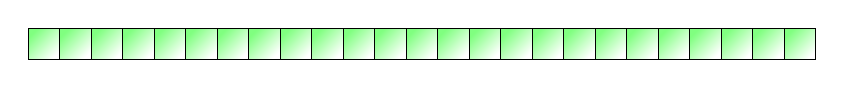
\begin{tikzpicture}[]
\foreach \x in {0.0, 0.4, ..., 9.6}
   \shadedraw [top color=green!50,shading angle=45] (\x,0) rectangle +(0.4,0.4);
\foreach \x in {0.2, 0.6, ..., 10.2}
   \node at (\x, 0.2) {{\scriptsize\kp}};  
\end{tikzpicture}
\end{center}

\begin{center}
\kpr
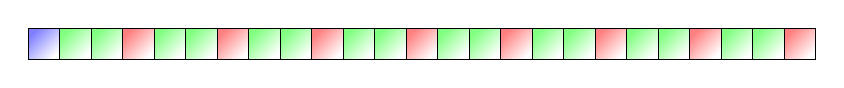
\begin{tikzpicture}[]
\foreach \x in {0.0, 0.4, ..., 9.6}
   \shadedraw [top color=green!50,shading angle=45] (\x,0) rectangle +(0.4,0.4); \shadedraw [top color=blue!50, shading angle=45] (0, 0) rectangle +(0.4,0.4);
\foreach \x in {1.2, 2.4, ..., 9.6}
   \shadedraw [top color=red!50,shading angle=45] (\x,0) rectangle +(0.4,0.4); \foreach \x in {0.2, 0.6, ..., 10.2}
   \node at (\x, 0.2) {{\scriptsize\kp}};  
\end{tikzpicture}
\end{center}

\begin{center}
\kpr
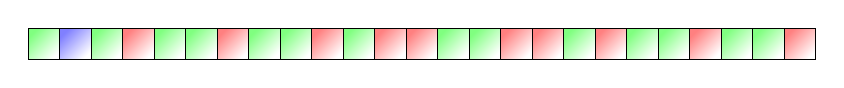
\begin{tikzpicture}[]
\foreach \x in {0.0, 0.4, ..., 9.6}
   \shadedraw [top color=green!50,shading angle=45] (\x,0) rectangle +(0.4,0.4); \shadedraw [top color=blue!50, shading angle=45] (0.4,0) rectangle +(0.4,0.4);
\foreach \x in {1.2, 2.4, ..., 9.6}
   \shadedraw [top color=red!50,shading angle=45] (\x,0) rectangle +(0.4,0.4);
\foreach \x in {2.4, 4.4, ..., 9.6}
   \shadedraw [top color=red!50,shading angle=45] (\x,0) rectangle +(0.4,0.4);
\foreach \x in {0.2, 0.6, ..., 10.2}
   \node at (\x, 0.2) {{\scriptsize\kp}};  
\end{tikzpicture}
\end{center}

\begin{center}
\kpr
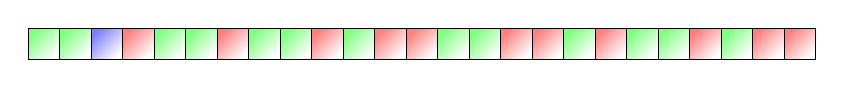
\begin{tikzpicture}[]
\foreach \x in {0.0, 0.4, ..., 9.6}
   \shadedraw [top color=green!50,shading angle=45] (\x,0) rectangle +(0.4,0.4); \shadedraw [top color=blue!50, shading angle=45] (0.8,0) rectangle +(0.4,0.4);
\foreach \x in {1.2, 2.4, ..., 9.6}
   \shadedraw [top color=red!50,shading angle=45] (\x,0) rectangle +(0.4,0.4);
\foreach \x in {2.4, 4.4, ..., 9.6}
   \shadedraw [top color=red!50,shading angle=45] (\x,0) rectangle +(0.4,0.4);
\foreach \x in {3.6, 6.4, ..., 9.6}
   \shadedraw [top color=red!50,shading angle=45] (\x,0) rectangle +(0.4,0.4); \foreach \x in {0.2, 0.6, ..., 10.2}
   \node at (\x, 0.2) {{\scriptsize\kp}};  
\end{tikzpicture}
\end{center}

\begin{center}
\kpr
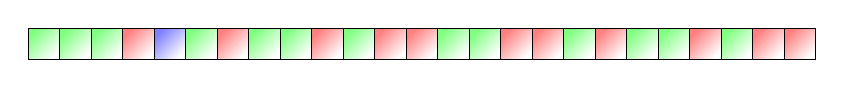
\begin{tikzpicture}[]
\foreach \x in {0.0, 0.4, ..., 9.6}
   \shadedraw [top color=green!50,shading angle=45] (\x,0) rectangle +(0.4,0.4); \shadedraw [top color=blue!50, shading angle=45] (1.6,0) rectangle +(0.4,0.4);
\foreach \x in {1.2, 2.4, ..., 9.6}
   \shadedraw [top color=red!50,shading angle=45] (\x,0) rectangle +(0.4,0.4);
\foreach \x in {2.4, 4.4, ..., 9.6}
   \shadedraw [top color=red!50,shading angle=45] (\x,0) rectangle +(0.4,0.4);
\foreach \x in {3.6, 6.4, ..., 9.6}
   \shadedraw [top color=red!50,shading angle=45] (\x,0) rectangle +(0.4,0.4); \foreach \x in {0.2, 0.6, ..., 10.2}
   \node at (\x, 0.2) {{\scriptsize\kp}};  
\end{tikzpicture}
\end{center}

\begin{center}
\kpr
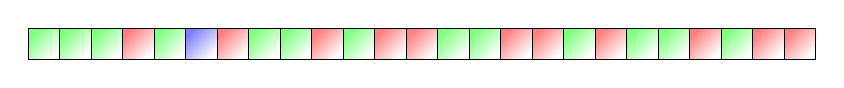
\begin{tikzpicture}[]
\foreach \x in {0.0, 0.4, ..., 9.6}
   \shadedraw [top color=green!50,shading angle=45] (\x,0) rectangle +(0.4,0.4); \shadedraw [top color=blue!50, shading angle=45] (2.0,0) rectangle +(0.4,0.4);
\foreach \x in {1.2, 2.4, ..., 9.6}
   \shadedraw [top color=red!50,shading angle=45] (\x,0) rectangle +(0.4,0.4);
\foreach \x in {2.4, 4.4, ..., 9.6}
   \shadedraw [top color=red!50,shading angle=45] (\x,0) rectangle +(0.4,0.4);
\foreach \x in {3.6, 6.4, ..., 9.6}
   \shadedraw [top color=red!50,shading angle=45] (\x,0) rectangle +(0.4,0.4); \foreach \x in {0.2, 0.6, ..., 10.2}
   \node at (\x, 0.2) {{\scriptsize\kp}};  
\end{tikzpicture}
\end{center}

\begin{center}
\kpr
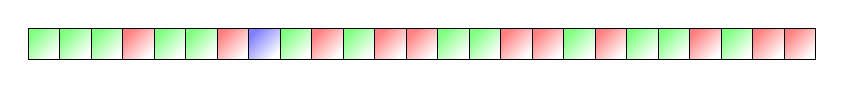
\begin{tikzpicture}[]
\foreach \x in {0.0, 0.4, ..., 9.6}
   \shadedraw [top color=green!50,shading angle=45] (\x,0) rectangle +(0.4,0.4); \shadedraw [top color=blue!50, shading angle=45] (2.8,0) rectangle +(0.4,0.4);
\foreach \x in {1.2, 2.4, ..., 9.6}
   \shadedraw [top color=red!50,shading angle=45] (\x,0) rectangle +(0.4,0.4);
\foreach \x in {2.4, 4.4, ..., 9.6}
   \shadedraw [top color=red!50,shading angle=45] (\x,0) rectangle +(0.4,0.4);
\foreach \x in {3.6, 6.4, ..., 9.6}
   \shadedraw [top color=red!50,shading angle=45] (\x,0) rectangle +(0.4,0.4); \foreach \x in {0.2, 0.6, ..., 10.2}
   \node at (\x, 0.2) {{\scriptsize\kp}};  
\end{tikzpicture}
\end{center}

This gives the primes (we add 2 to the beginning of the list):
\resizebox{\textwidth}{!}{
\begin{tabular}{ccccccccccccccc}
2&3&5&7&11&13&17&19&23&29&31&37&41&43&47
\end{tabular}}
\end{frame}

\begin{frame}
\frametitle{The Sieve of Eratosthenes: In C}
\begin{itemize}
\item When implementing this in C it makes sense to use a bit to indicate `primeness' of a number.
\item The smallest addressable unit of memory in C is the {\tt \kw{char}} which consists of 8 bits.
\item We therefore need to perform \emph{masking} to isolate individual bits.
\end{itemize}
\begin{block}{Masking}
We access the $j^\mathrm{th}$ bit of a variable {\tt x} as follows:
\begin{center}
\begin{tabular}{l l}
\tt \kw{if}(x \& (1 << j))&Check to see if it's set\\
\tt x |= (1 << j)& To set the bit\\
\tt x \&= $\sim$(1 << j)&To clear the bit
\end{tabular}
\end{center}
\end{block}
\end{frame}

\begin{frame}[fragile]
\frametitle{The Sieve of Eratosthenes: Implementation}
\vspace{-0.2in}
\begin{semiverbatim}
\scriptsize
\kr\kl\kw{void} findPrimes(NUM_TYPE * Prime_List, \kw{int} max_num)
\kl\{
\kl   \kw{int} current_num = 3;
\kl   NUM_TYPE Mask=1;
\kl
\kl   \kw{while}(current_num*current_num <= max_num)
\kl   \{
\kl      \kw{int} Pnum = current_num/(2 * BITS_PER_NUM);
\kl      \kw{int} Pbit = (current_num-Pnum * 2 * BITS_PER_NUM)/2;
\kl      \kc{/* Current Number is prime so strike out multiples */}
\kl      \kw{if}(~Prime_List[Pnum] & (Mask <<Pbit))
\kl      \{
\kl         \kw{int} strike = current_num * current_num;
\kl         \kw{while}(strike <= max_num)
\kl         \{
\kl            \kw{int} Snum = strike/(2*BITS_PER_NUM);
\kl            \kw{int} Sbit = (strike - Snum * 2 * BITS_PER_NUM)/2;
\kl            Prime_List[Snum] |= (Mask << Sbit);
\kl            strike += 2 * current_num;
\kl         \}                       
\kl      \}
\kl      current_num += 2;
\kl   \}
\kl\}
\end{semiverbatim}
\end{frame}

\begin{frame}[fragile]
\frametitle{The Sieve of Eratosthenes : Printing out the Primes}
\begin{semiverbatim}
\small
\kr\kl\kw{void} printPrimes(NUM_TYPE * Prime_List, \kw{int} max_num)
\kl\{
\kl   \kw{int} i;
\kl   NUM_TYPE Mask=1;
\kl
\kl   \kw{for}(i = 3;i <= max_num;i = i+2)
\kl   \{
\kl      \kw{int} Pnum=i/(2*BITS_PER_NUM);
\kl      \kw{int} Pbit=(i-Pnum*2*BITS_PER_NUM)/2;
\kl      \kw{if} (~Prime_List[Pnum] & (Mask <<Pbit))
\kl         printf(\kt{"\%d\\n"}, i);
\kl   \}
\kl\}
\end{semiverbatim}
\end{frame}

\section{Projects}
\subsection{Compiling from Multiple Files}
\begin{frame}
\frametitle{Projects and Makefiles}
\begin{itemize}
\item It is possible (and encouraged) to build a program from multiple {\tt .c} files.
\item This maximises the portability of the code, and
\item Speeds up compiling - if we only change one {\tt .c} file we only need to recompile one file...
\item Visual Studio manages programs in to so-called \emph{projects}, and everything is done graphically.
\item UNIX systems have a very powerful program called {\tt make} which manages projects. Information for building programs is stored in a {\tt Makefile}.
\end{itemize}
\end{frame}

\begin{frame}[fragile]
\frametitle{A sample {\tt Makefile}}
\framesubtitle{There are many ways of writing one, this is mine!}
\begin{exampleblock}{}
\begin{semiverbatim}
\scriptsize
CFLAGS = -O2 -DNDEBUG -Wall -ansi
LFLAGS = -lm
CC = gcc
CLEANFILES = crypticc.o matrixfunctions.o cryptic cryptic.exe

cryptic: crypticc.o matrixfunctions.o
         \$(CC) crypticc.o matrixfunctions.o \$(LFLAGS) -o cryptic
         
clean:
        touch \$(CLEANFILES)
        rm \$(CLEANFILES)
\end{semiverbatim}
\end{exampleblock}
\begin{itemize}
\item This compiles {\tt crypticc.c} and {\tt matrixfunctions.c}.
\item It then links them to produce {\tt cryptic.exe} (Cygwin) or {\tt cryptic} (UNIX).
\item It has two rules {\tt cryptic} (default) to build the program and {\tt clean} to clean up all the compiled output.
\end{itemize}
\end{frame}

\begin{frame}
\frametitle{The C Preprocessor - How to {\tt\#define} Externally}
We are not restricted to {\tt \kw{\#define}} statements in source code.
\begin{block}{Visual Studio}
In the Visual Studio ``project properties'' $\rightarrow$ ``C/C++'' $\rightarrow$ ``Preprocessor'' option we can specify preprocessor definitions.
\end{block}

\begin{block}{gcc}
In gcc we can specify define statements in the command line as follows:\\
{\tt gcc myfile.c -DNDEBUG -o myprogram }
\end{block}
\end{frame}


\section{Function Pointers}
\subsection{Pointers IV - Functions Pointers}
\begin{frame}[fragile]
\frametitle{More Pointers!}
\begin{itemize}
\item So far, we have seen examples of pointers to:
\begin{itemize}
\item native types (such as {\tt\kw{int}*}, {\tt\kw{float}*}, {\tt\kw{double}*}...),
\item something unknown ({\tt\kw{void}*}),
\item structures (such as {\tt FILE*}),
\item and pointers themselves (such as {\tt\kw{int}**}, {\tt\kw{double}**}...).
\end{itemize}
\item There is one more pointer type, a pointer to a \emph{function}.
\end{itemize}

\begin{block}{Why point to functions?}
C code is often re-used between projects. Mathematical routines such as ones to find roots of functions, become extremely limited if they are tied down to a specific case.
\end{block}

\begin{exampleblock}{Declaring a pointer to a function}
One way is to use a {\tt\kw{typedef}}:
\vspace{-0.1in}
\begin{center}
\tt \kw{typedef} \kw{double} (* fx)(\kw{double} x);
\end{center}
\end{exampleblock}
\end{frame}

\subsection{Example of a Function Pointer}
\begin{frame}[fragile]
\frametitle{Function Pointers - An example}
\vspace{-0.2in}
\begin{semiverbatim}
\tiny
\kw{\#include} \kt{<stdio.h>}
\kw{typedef double} (* fx)(\kw{double} x);

\kw{double} newtonSolve(fx func, fx grad, \kw{double} guess)
\{
   \kw{unsigned int} loop;
   \kw{for} (loop = 0; loop < 10; loop++) guess -=func(guess)/grad(guess);
   \kw{return} guess;
\}

\kw{double} sample(\kw{double} x)
\{
   \kw{return} x*x-2.0;
\}

\kw{double} dsample(\kw{double} x)
\{
   \kw{return} 2.0*x;
\}

\kw{int} main()
\{
   \kw{double} sol = newtonSolve(sample, dsample, 1.0);
   printf(\kt{"Solution = \%.15lg\\n"}, sol);     
   printf(\kt{"Residue = \%lg\\n"}, sample(sol));
   \kw{return} 0;
\}
\end{semiverbatim}
This should get you started with exercise \# 5.
\end{frame}

\section{Using Existing Code}
\subsection{Don't Do it All Yourself!}
\begin{frame}
\frametitle{Don't Do it All Yourself!}
\begin{itemize}
\item As you have seen from the exercises, writing functions to solve equations such as cubics can become complicated (especially when rounding error needs to be minimised).
\item A lot of people have spent a considerable amount of time attempting to perfect implementations of mathematical functions.
\item Routines written by a third party are packaged in \emph{libraries}.
\end{itemize}
\end{frame}

\subsection{Converting Fortran}
\begin{frame}
\frametitle{Using Fortran Code}
\begin{itemize}
\item Good news! Scientific programming has been going on for over 60 years (counting from Colossus) in Britain.
\item Unfortunately a lot of this has been carried out in Fortran.
\end{itemize}
\begin{block}{\tt f2c}
Bell Labs have released a program called {\tt f2c} which converts Fortran source code to C. The output from {\tt f2c} is usually not very human friendly, but it does at least compile.
\end{block}
\end{frame}

\subsection{Scientific Libraries}
\begin{frame}
\frametitle{GNU Scientific Library - GSL}
GNU have released their C Scientific Library:
\begin{center}
\url{http://www.gnu.org/software/gsl/}
\end{center}

\begin{itemize}
\item It is managed by scientists at Los Alamos, and is very comprehensively documented.
\item GSL requires gcc (for Windows users, Cygwin can be used).
\end{itemize}

\begin{alertblock}{Licensing}
``GSL can be used internally ("in-house") without restriction, but only redistributed in other software that is under the GNU GPL.''
\end{alertblock}
\end{frame}

\begin{frame}[fragile]
\frametitle{GSL Example}
\vspace{-0.2in}
\begin{semiverbatim}
\small
\kw{\#include} \kt{<stdio.h>}
\kw{\#include} \kt{<gsl/gsl\_sf\_bessel.h>}

\kw{int} main()
\{
   \kw{double} x = 0.0;

   printf(\kt{"Enter x \\n"});
   scanf(\kt{"\%lf"}, \&x);
   printf(\kt{"J0(\%g) = \%.18e\\n"}, x, gsl\_sf\_bessel\_J0(x));

   return 0;
\}
\end{semiverbatim}
Compile this using the command-line:
\begin{alertblock}
\tt gcc gsl-sample.c -lgsl  -lgslcblas -lm -o gsl-sample
\end{alertblock}
\end{frame}

\begin{frame}
\frametitle{NAGLIB}
The Numerical Algorithms Group, based in Oxford, maintain a software library called NAGLIB.
\begin{itemize}
\item Imperial College have signed a site license for NAGLIB.
\item It can be installed on departmental machines upon request.
\item You are allowed to install it on your home machines.
\end{itemize}
\end{frame}

\begin{frame}
\frametitle{General Numerical Software}
\begin{center}
\begin{columns}
\begin{column}{0.3\textwidth}

\includegraphics[width=\textwidth]{netlib.png}\\
\end{column}
\end{columns}
The Netlib Repository contains a lot of very useful numerical codes and papers. It is definitely worth having a route through their website:\\
\url{www.netlib.org}
\end{center}
\end{frame}

\section{Parallel Computing}
\subsection{High Performance Computing}
\subsection{Multi-Threading}

\section{Other Programming Languages}
\subsection{C++}
\begin{frame}
\frametitle{Moving on to C++}
\begin{block}{What is it?}
\begin{itemize}
\item C++ can be thought of very loosely as an object oriented extension to C.
\item The C++ standard is over twice as big as the C standard.
\item C++ is in the process of changing (at the time of writing C++0x is being adopted by compilers).
\end{itemize}
\end{block}
\begin{exampleblock}{References}
\begin{columns}
\begin{column}{1.7cm}
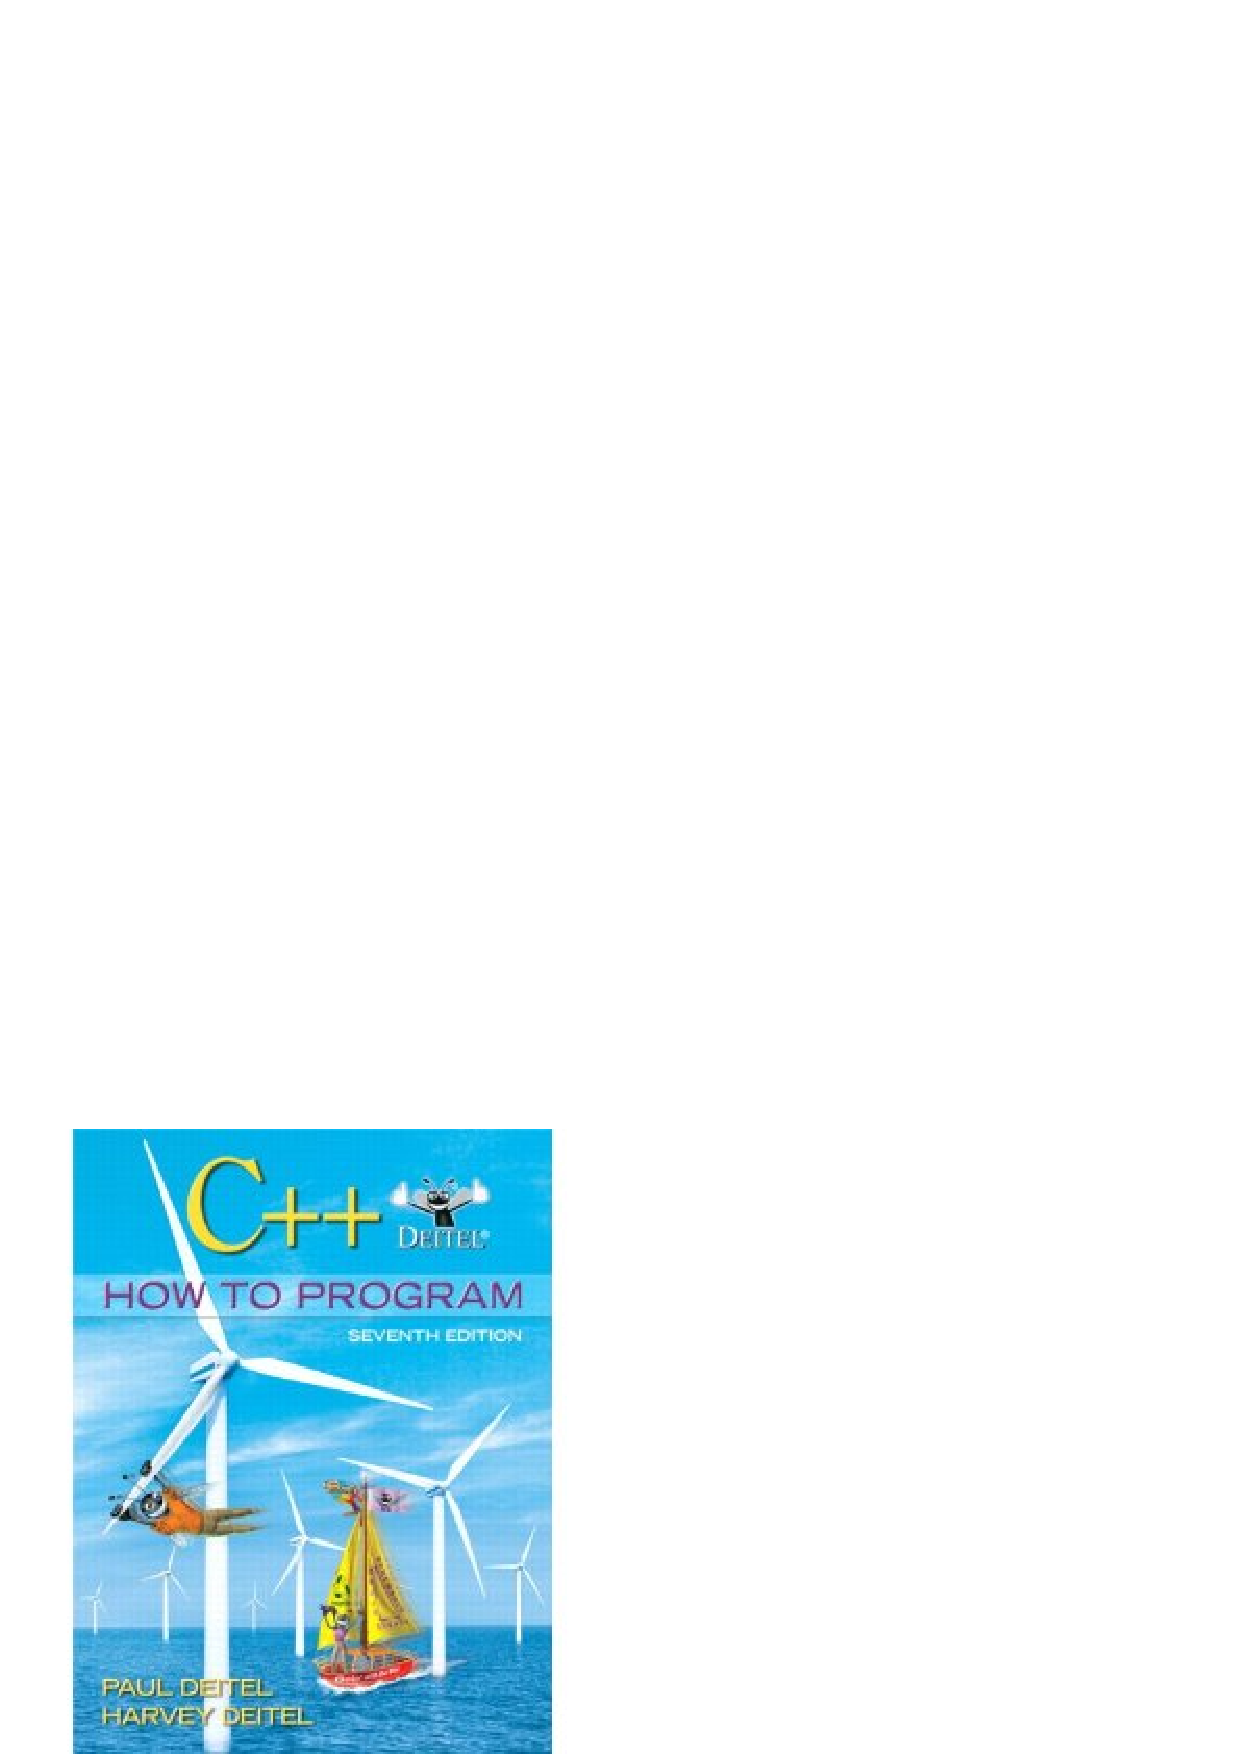
\includegraphics[width=\textwidth]{deitelnew.jpg}
\end{column}
\begin{column}{8cm}
\begin{itemize}
\item One good book that has been brought to my attention is ``C++ How to Program 7th Edition'' by Harvey and Paul Deitel published in 2010.
\item Before buying any C++ book, make sure that it is recent, and that you like the writing style.
\end{itemize}
\end{column}
\end{columns}
\end{exampleblock}
\end{frame}

\subsection{C\#}
\begin{frame}
\frametitle{Moving on to C\# (or Java)?}
Java and C\# belong to a different class of language.
\begin{columns}
\begin{column}{0.55\textwidth}
\begin{itemize}
\item Java and C\#, both target \emph{virtual machines}.
\item Pointers are hidden from the user in C\# and completely absent from Java.
\item Most memory allocation and de-allocation is done automatically, via
\emph{garbage collection}.
\item Java code can target multiple platforms,
C\# is supported only on Microsoft platforms.
\end{itemize}
\end{column}
\begin{column}{0.7\textwidth}
\hspace{-0.57in}\rlap{\includegraphics[width=\textwidth]{comparison}}
\end{column}
\end{columns}
\end{frame}

\begin{frame}
\frametitle{C\# References}
\begin{block}{Book}
\begin{columns}
\begin{column}{1.7cm}
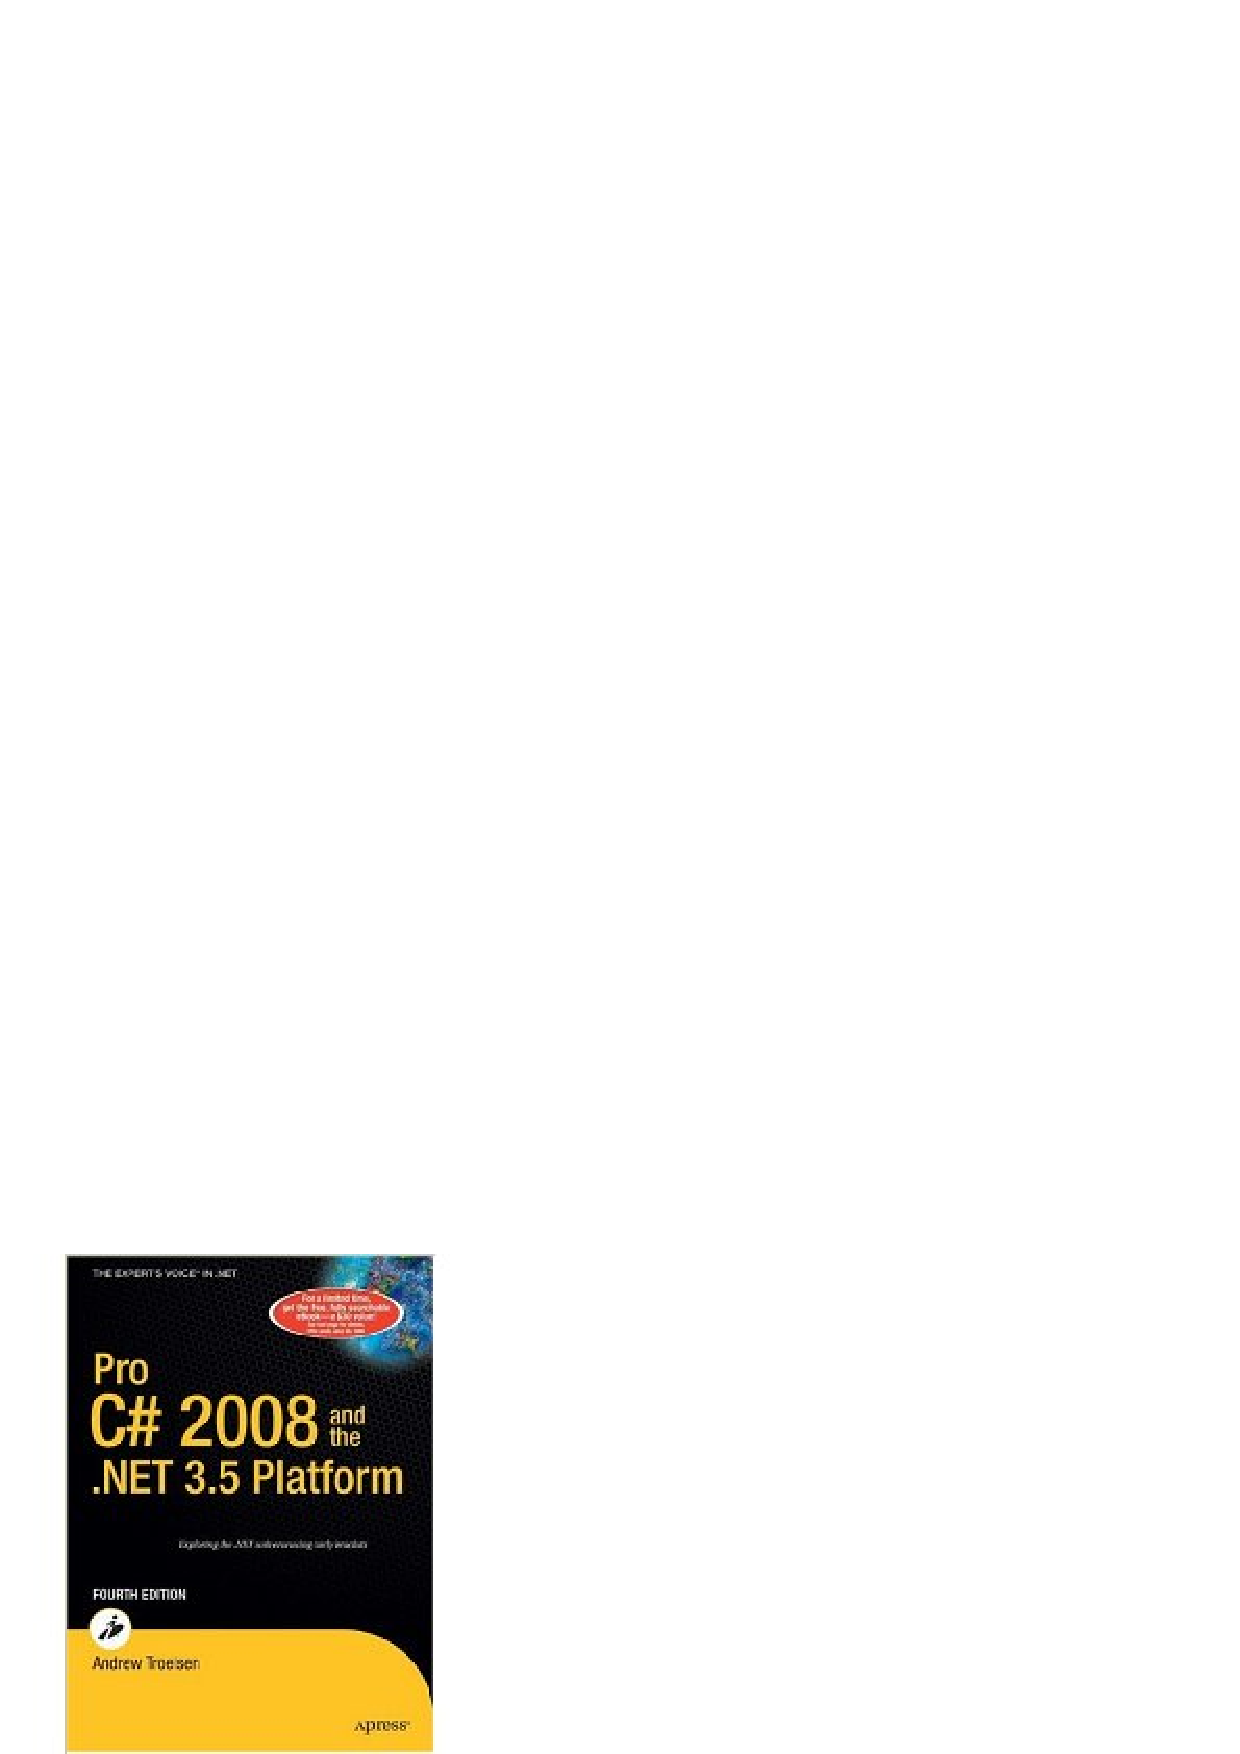
\includegraphics[width=\textwidth]{csharp.png}
\end{column}
\begin{column}{0.8\textwidth}
\begin{itemize}
\item ``Pro C\# 2008 and the .NET 3.5 Platform, Fourth Edition'' by Andrew Troelsen,
appears to be up-to-date and comprehensive.
\item I would recommend you skim through a copy before buying. (.Net 4.0 is 2 weeks away).
\end{itemize}
\end{column}
\end{columns}
\end{block}
\begin{exampleblock}{MSDN}
The definitive (and free) source of information for Microsoft Platforms is the MSDN, the C\# documentation is browsable at:\\
{\small\url{http://msdn.microsoft.com/en-gb/library/kx37x362.aspx}}
\end{exampleblock}
\end{frame}


\section{EXCLUDE}
\subsection{INTERNATIONAL CHAR}
\begin{frame}[fragile]
\frametitle{Internationalisation (i18n)}
There are two methods that C employs to overcome the limitations of {\tt \kw{char}}:
\begin{block}{Wide Characters \& Wide Strings (used in Windows)}
C has a wide character type called {\tt \kw{wchar\_t}}, a capital L is used to denote a wide character or wide string:
\vspace{-0.1in}
\begin{semiverbatim}
\kw{wchar_t} mwchar = L\kt{'a'};
\kw{wchar_t} * wideString = L\kt{"A wide string"};
\end{semiverbatim}
\end{block}

\begin{block}{Multibyte Characters (used in Linux)}
Another trick is to encode frequently used characters (such as numbers and Roman letters) using ASCII as normal, and for larger character sets (such as Hanzi) combine two or more {\tt \kw{char}}s together.
\end{block}
\end{frame}

\begin{frame}[fragile]
\frametitle{Unicode Sample}
\framesubtitle{A sample to convert from wide to multibyte, then print}
\vspace{-0.1in}
\begin{semiverbatim}
\tiny
\kr\kl\kw{\#include} \kt{<stdio.h>}
\kl\kw{\#include} \kt{<wchar.h>}
\kl\kw{\#include} \kt{<stdlib.h>}
\kl\kw{\#include} \kt{<locale.h>}
\kl
\kl\kw{int} main()
\kl\{
\kl   \kw{wchar_t} * unicodeString = L\kt{"a name:\\x8FEA\\x6587\\nMaths symbols:"}
\kl                             L\kt{"x\\x220A\\x2115\\x2204\\x222B\\x2202\\n"};
\kl   \kw{char} * mbString = NULL;
\kl   size\_t mbSize;
\kl   \kc{/* select native locale */}
\kl   \kw{char} * locale = setlocale( LC\_CTYPE, \kt{""});
\kl   printf(\kt{"MB\_CUR\_MAX = \%d\\n"}, MB\_CUR\_MAX);
\kl   printf(\kt{"sizeof(wchar\_t) = \%d\\n"}, \kw{sizeof}(\kw{wchar\_t}));
\kl   printf(\kt{"locale = \%s\\n"}, locale);
\kl
\kl   mbSize = (wcslen(unicodeString)+1)*MB\_CUR\_MAX;
\kl   mbString = (\kw{char} *) malloc(mbSize);
\kl   \kw{if} (!mbString)
\kl   \{
\kl      fprintf(stderr, \kt{"Unable to allocate multibyte buffer"});
\kl      \kw{return} -1;
\kl   \}
\kl
\kl   wcstombs(mbString, unicodeString, mbSize);
\kl   printf(\kt{"Multibyte: \%s\\n"}, mbString);
\kl   free(mbString); 
\kl   \kw{return} 0;
\kl\}
\end{semiverbatim}
\end{frame}

\begin{frame}
\frametitle{Multibyte Output}
\begin{itemize}
\item Logging in to a Linux box via PuTTY and using UTF-8 encoding, I get:
\begin{center}
\includegraphics[width=0.5\textwidth]{unicode.PNG}
\end{center}
\item This won't work properly for the Windows text console, as it doesn't allow for any unicode encodings. (If you set both the system and user locales to Chinese, then the Hanzi will display properly).
\end{itemize}
\end{frame}

\subsection{GRAPHICS}
\begin{frame}
\frametitle{JPEG Manipulation}
\begin{itemize}
\item The Independent JPEG Group, release a freeware JPEG (compressor/decompressor) library.
\item Code is available from \url{http://www.ijg.org}; the most recent version as of writing is 8a (dated 28-Feb-2010).
\item To use the code in Visual Studio one needs to rename some project files (please refer to {\tt install.txt} for details).
\item Example code is included that demonstrates the proper use of the library, for an example of decompression please refer to {\tt djpeg.c}.
\end{itemize}


\end{frame}

\begin{frame}
\frametitle{Graphics Programming in C}
\begin{alertblock}{Avoid it if you can!}
Most of the time scientific output can be plotted quite well by GNUplot, Maple and Matlab.
\end{alertblock}
\begin{block}{If you still want to...}
\begin{columns}
\begin{column}{1.7cm}
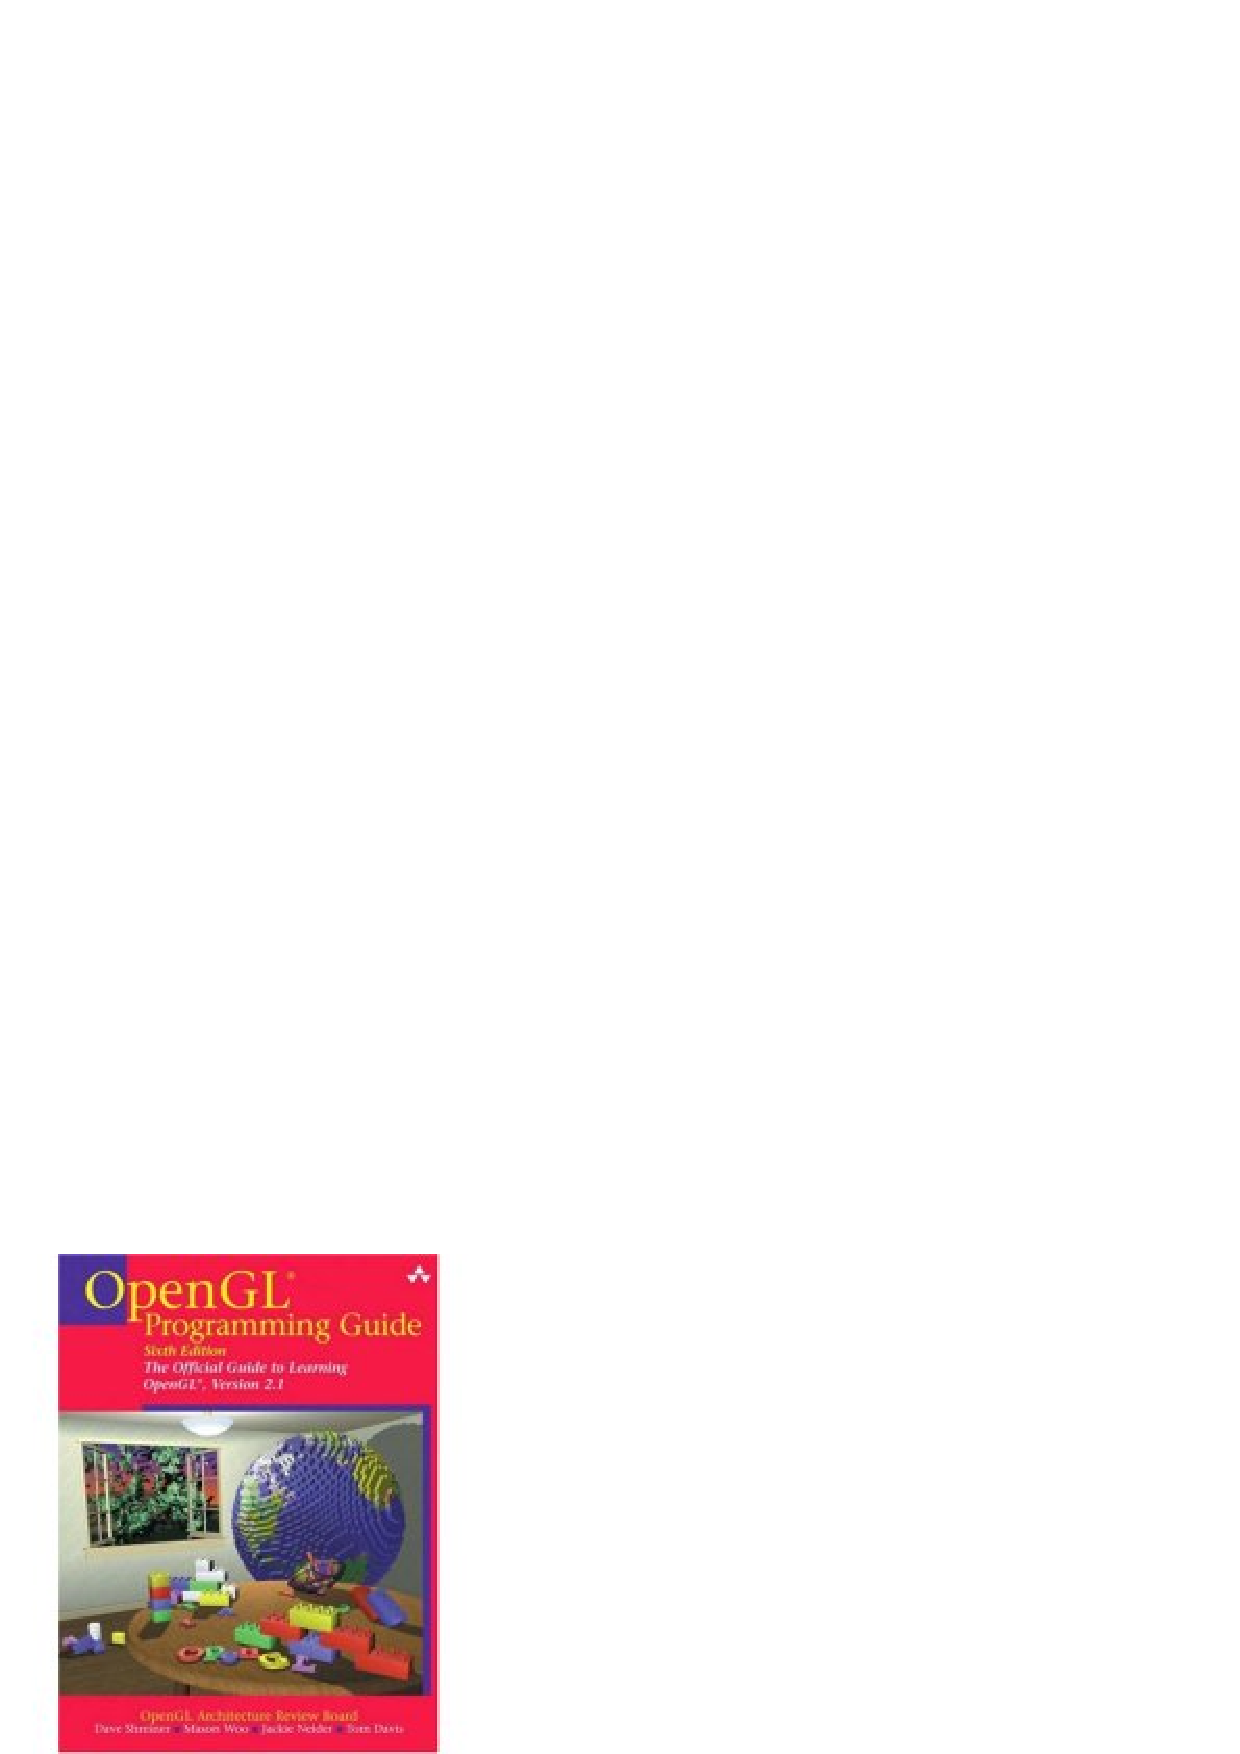
\includegraphics[width=\textwidth]{opengl.png}
\end{column}
\begin{column}{8cm}
I recommend that you program in OpenGL as it is portable across architectures and makes use of the graphics hardware in machines. I learnt OpenGL from the ``Red Book''; OpenGL Programming Guide: The Official Guide to Learning OpenGL.
\end{column}
\end{columns}
\end{block}
\begin{exampleblock}{Example Code}
I have placed an OpenGL sample on my website, it also conveniently demonstrates almost all the C we have covered in this course!
\end{exampleblock}
\end{frame}
\subsection{FORTRAN}
\begin{frame}[fragile]
\frametitle{Calling Fortran from C - the C {\tt main} function}
\begin{semiverbatim}
\small
\kw{\#include} \kt{<stdio.h>}

\kw{extern double} ffunc01_(\kw{double} *x);

\kw{double} callfortran(\kw{double} x)
\{
   \kw{return} ffunc01_(&x);
\}

\kw{int} main()
\{
   \kw{double} x = 1.0;
   
   printf(\kt{"Hello from C!\\n"});
   printf(\kt{"fsub(\%g) = \%g\\n"}, x, callfortran(x));
   \kw{return} 0;
\}
\end{semiverbatim}
\end{frame}

\begin{frame}[fragile]
\frametitle{Calling Fortran from C - The Fortran Function}
\begin{semiverbatim}
\small
\kw{function} ffunc01(x)
   \kw{real}(\kw{kind}=8), \kw{intent}(\kw{in}) :: x
   \kw{real}(\kw{kind}=8)             :: ffunc01
   
   ffunc01 = 10*x + 1   
   print *, \kt{'In fortran, received x = '}, x
   print *, \kt{'returning'}, ffunc01   
\kw{end function}
\end{semiverbatim}
\begin{itemize}
\item We explicitly specify {\tt kind=8}, i.e. {\tt double} precision.
\item In {\tt g95}, all exported functions have a trailing underscore.
\item Fortran arguments to functions are pointers.
\end{itemize}
\end{frame}

\begin{frame}[fragile]
\frametitle{Calling C from Fortran - Fortran Interface}
\begin{semiverbatim}
\scriptsize
\kw{module} cmodule
   \kw{implicit none}
\kw{contains}

   \kw{function} my_func(x)
      \kw{real}, \kw{intent}(\kw{in}) :: x
      \kw{real}             :: my_func
      \kw{real}(\kw{kind}=8)     :: tmp
            
      \kw{interface}
         \kw{function} cfunc01(x)
            \kw{real}(\kw{kind}=8), \kw{intent}(\kw{in}) :: x
            \kw{real}(\kw{kind}=8)             :: cfunc01
         \kw{end function} cfunc01
      \kw{end interface}
      
      tmp = x
                  
      my_func = cfunc01(tmp)
   \kw{end function} my_func
\kw{end module} cmodule
\end{semiverbatim}
\end{frame}

\begin{frame}[fragile]
\frametitle{Calling C from Fortran - Fortran entry point}
\begin{semiverbatim}
\small
\kw{program} test
   \kw{use} cmodule
   \kw{implicit none}
   
   \kw{real} :: myx = 26.0980
   
   print *, \kt{'myx = '}, myx
   print *, \kt{'my_funx(myx) = '}, my_func(myx)
\kw{end program}
\end{semiverbatim}
\begin{itemize}
\item We must compile the {\tt cmodule} \emph{before} the entry point.
\item This is due to Fortran .mod files (think auto-generated .h files).
\end{itemize}
\end{frame}

\begin{frame}[fragile]
\frametitle{Calling C from Fortran - The C function}
\begin{semiverbatim}
\scriptsize
\kw{\#include} \kt{<stdio.h>}

\kw{double} cfunc01_(\kw{double} * x)
\{
   \kw{double} retval = (*x)*(*x) - 1.0;
   printf(\kt{"In cfunc01(): received x = %g, returning: %g\\n"},
          *x, retval);
   \kw{return} retval;
\}
\end{semiverbatim}
\begin{itemize}
\item The arguments to the c function are pointers.
\item {\tt cfunc01} is referenced from the {\tt cmodule} interface.
\item We add a trailing underscore to the function name.
\item Function name translation in object files is known as \emph{name mangling}.
\end{itemize}
\begin{alertblock}{}
\begin{center}
Different compilers have different calling conventions!
\end{center}
\end{alertblock}
\end{frame}

\begin{frame}[fragile]
\frametitle{Linking Fortran and C - Putting it all together}
\begin{exampleblock}{}
\begin{semiverbatim}
\scriptsize
.SUFFIXES: .f90
CFLAGS = -pedantic -ggdb -Wall -ansi
FFLAGS = -ggdb
LFLAGS = -lm
CC = gcc
F90 = g95
CLEANFILES = fmain.o csub.o demo1 fmod.o cmodule.mod demo1.exe \\
             cmain.o demo2 demo2.exe ffunc.o

all:    demo1 demo2

demo1:  cmain.o ffunc.o
        \$(F90) cmain.o ffunc.o -o demo1

demo2:  fmod.o fmain.o csub.o
        \$(F90) fmod.o fmain.o csub.o -o demo2
 
clean:
        touch \$(CLEANFILES)
        rm \$(CLEANFILES)

.f90.o:
        \$(F90) \$(FFLAGS) -c \$*.f90
\end{semiverbatim}
\end{exampleblock}
\end{frame}

\begin{frame}[fragile]
\frametitle{Running the codes}
Running the first demo:
\begin{semiverbatim}
\small
\$ ./demo1 
Hello from C!
 In fortran, received x =  1.  returning 11.
fsub(1) = 11
\end{semiverbatim}

and the second demo:
\begin{semiverbatim}
\small
\$ ./demo2 
 myx =  26.098
In cfunc01(): received x = 26.098, returning: 680.106
 my\_funx(myx) =  680.1056
\end{semiverbatim}
\end{frame}

\section{CRYPTIC C}
\subsection{work on}
\begin{frame}[fragile]
\frametitle{Cryptic C - What do I do?}
\begin{semiverbatim}
\scriptsize
\kr\kl\kw{void} whatdoIdo(\kw{double} *A, \kw{double} * B, \kw{double} *C,
\kl                    \kw{unsigned int} L, \kw{unsigned int} M,
\kl                    \kw{unsigned int} N)
\kl\{
\kl   \kw{unsigned int} i, k;
\kl   \kw{double} temp, *bptr, *bend, *cptr;
\kl
\kl   \kw{for}(i=0; i < L; i++)
\kl   \{
\kl      \kw{for} (k=0; k < M; k++)
\kl      \{
\kl         temp = A[i*M+k];
\kl         cptr = &C[i*N];
\kl         bptr = &B[k*N];
\kl         bend = &B[(k+1)*N];
\kl         \kw{while} (bptr < bend)
\kl            *cptr++ += temp*(*bptr++);
\kl      \}
\kl   \}
\kl\}
\end{semiverbatim}
\end{frame}

\end{document}




